\chapter{System Analysis and Design}

\section{Architecture Overview}
    This project's architecture is designed not only to be flexible, but also to maximize the performance result. There are three components in this project; server side, client side, and the database. The client side is the web browser. The server side provides API service for the client side and also connects to the database which is MongoDB in this case.
    
    \vspace{25mm}
    \FloatBarrier
    	\begin{figure}[h!]
            \centering
                % can use width=\linewidth
        		\includegraphics[width=10cm]{images/chapter-03/architecture.png}
        		\caption{Architecture Overview}
        \end{figure}
	\FloatBarrier

\clearpage
\section{Use Case Diagram}
    % only super admin can see individual
    % uploader = can upload
    %user = 
    %hiv coordinator = can see individual only their hosp
    
    We have been gathering requirements from ministry of public health team, we found that there are four main types of user which are super admin, user, HIV coordinator, and up-loader. 
    
    User can log-in to EIIS system, by filling user-name and password, and log-out. User role can see at a glance report, demographics report, upload status page and workload report as shown in figure \ref{use-case}.
    
    
    Super admin can can do everything that User can do, and also see all the individual report which it contains the sensitive information of the patient. For example, id, hospital number codes of the patient, and so on as shown in figure \ref{use-case}. 
    
    
    \FloatBarrier
    	\begin{figure}[h!]
            \centering
                % can use width=\linewidth
        		\includegraphics[width=12cm]{images/chapter-03/UseCaseDiagram.png}
        		\caption{Use Case Diagram}
        		\label{use-case}
        \end{figure}
	\FloatBarrier
	
	Like super admin, HIV coordinator can see the individual report, but they can see only the individual report of their responsibility hospitals. It means that they can see only a group of patient that have a record on that hospital. Unlike other roles, uploader can upload file in and file out to this web-application as shown in figure \ref{use-case2}.
	
	\vspace{15mm}
	\FloatBarrier
    	\begin{figure}[h!]
            \centering
                % can use width=\linewidth
        		\includegraphics[width=12cm]{images/chapter-03/UseCaseDiagram2.png}
        		\caption{Use Case Diagram}
        		\label{use-case2}
        \end{figure}
	\FloatBarrier
	
\clearpage
\section{Activity Diagram}

    \subsection{Log-In}
    % Log-in
    All users role can log in to the EIIS system. All processes to log in are simple. First, they need to fill in user name and password as it shown in figure \ref{log-in}, and after they finish fill in, they just click log-in in order to log-in. If the process is success, it will bring you to the system. If the process is failure, it will warn you that you put the wrong user name or password. The steps of logging-in is shown in figure \ref{log-in-activity-diagram}. 

    \vspace{10mm}
    \FloatBarrier
    	\begin{figure}[h!]
            \centering
                % can use width=\linewidth
        		\includegraphics[width=9cm]{images/chapter-03/logIn_logOut.png}
        		\caption{Log-In}
        		\label{log-in-activity-diagram}
        \end{figure}
	\FloatBarrier
	%Upload
	
	
	\subsection{Upload} \label{upload_file_activity_diagram}
	Only uploader role can upload the file to the system. There are two main steps to upload the file. First, uploader need to choose hospital, month, and year, then click confirm to go to the next step as it shown in figure \ref{upload-status1}. Second, uploader need to choose either file-in or file-out then click upload. If upload process is success, then the upload process is end. If upload process is failure, then uploader have to make sure that they have to choose either file-in or file-out in order to upload as it shown in figure \ref{upload-status2}. If upload fail, it will warn the user as it shown in figure \ref{upload-error}. The steps of uploading is shown in figure \ref{activity_upload}.
	
	\FloatBarrier
    	\begin{figure}[h!]
            \centering
                % can use width=\linewidth
        		\includegraphics[width=6cm]{images/chapter-03/Upload.png}
        		\caption{Upload}
        		\label{activity_upload}
        \end{figure}
	\FloatBarrier
	
	%check upload status
	\subsection{Checking Upload Status} \label{check_upload_status_activity_diagram}
	All users can check the upload status. The steps to check upload status is simple as log-in. First, user need to choose type of report, area, province, and year then click search to see the upload status as it shown in figure \ref{upload-status0}. The steps of checking upload status is shown in figure \ref{check-upload-status}.
	
	\FloatBarrier
    	\begin{figure}[h!]
            \centering
                % can use width=\linewidth
        		\includegraphics[width=10cm]{images/chapter-03/Upload_status.png}
        		\caption{Check Upload Status}
        		\label{check-upload-status}
        \end{figure}
	\FloatBarrier
	
	%At a Glance Report
	\subsection{At a Glance Report} \label{at_a_glance_report}
	All users can see a glance report, and the process to see the report is not complex as in figure \ref{glance-report}. In order to see the report, user need to choose disease, criteria of that disease, times , and types of report area as it shown in figure \ref{at-a-glance-report}. There are three types of time that user can choose which are all time, range time, and end-point. If user select all time, it means that user select the time from the beginning to the end of the data. If user select range time, it means that user need to select the beginning month and year and the end month and year time by themselves. If the user select end-point time, it means that user need to select the endpoint month and year time. In addition, there are four scope of choosing type of report which are all, area, province, and hospital. In this field, if user choose all scope, it means all the data. If user choose area scope, it means that user have to choose specific area. Like area, if user choose province scope, it means that user have to choose specific area first then it will filter the provinces of that area, and user need to choose province. If user choose hospital scope, then user need to choose area, province, and hospital. If you want to see all the select user interface, you can see in section \ref{filter-data}. The steps of requesting at a glance report is shown in figure \ref{glance-report}
	
	\FloatBarrier
    	\begin{figure}[h!]
            \centering
                % can use width=\linewidth
        		\includegraphics[width=\linewidth]{images/chapter-03/atAGlance.png}
        		\caption{At a Glance Report}
        		\label{glance-report}
        \end{figure}
	\FloatBarrier
	
	%Demographics Report
	\subsection{Demographics Report} \label{demographics_report_sec}
	All users can see a demographics report, and the process is close to the process to see a glance report as the user interface of demographics report is shown in figure \ref{demographics-report}. In order to see the report, user need to choose nation, disease, criteria of that disease, times , and types of report area.There are three types of time that user can choose which are all time, range time, and end-point. If user select all time, it means that user select the time from the beginning to the end of the data. If user select range time, it means that user need to select the beginning month and year and the end month and year time by themselves. If the user select end-point time, it means that user need to select the endpoint month and year time. In addition, there are four scope of choosing type of report which are all, area, province, and hospital. In this field, if user choose all scope, it means all the data. If user choose area scope, it means that user have to choose specific area. Like area, if user choose province scope, it means that user have to choose specific area first then it will filter the provinces of that area, and user need to choose province. If user choose hospital scope, then user need to choose area, province, and hospital. If you want to see all the select user interface, you can see in section \ref{filter-data}. The steps of requesting demographics report is shown in figure \ref{demographics}
	
	
	 \FloatBarrier
    	\begin{figure}[h!]
            \centering
                % can use width=\linewidth
        		\includegraphics[width=\linewidth]{images/chapter-03/Demographics.png}
        		\caption{Demographics Report}
        		\label{demographics}
        \end{figure}
	\FloatBarrier
	
	%Individual Report
 	\subsection{Individual Report}
 	\label{individual_report_activity_diagram}
 	Only HIV coordinator and super admin roles that can view individual report. There is only 1 main step in order to see individual patient information. That step is to click "see information" at the last column of that row that contain the CID of the patient you want to view their information. Moreover, at the first page of individual report it can only contain 50 patients, so there will be previous and next bottom for look up the rest of patients. At individual report there is also a back button where you can click and go back to first step in order to look at another individual patient information. The steps of requesting individual report is shown in figure \ref{individual-report} However, for the user interface is the work that we will reimplemented in the future.
 	
 	\FloatBarrier
     	\begin{figure}[h!]
            \centering
                 % can use width=\linewidth
         		\includegraphics[width=9cm]{images/chapter-03/individual_report.png}
         		\caption{Individual Report}
        		\label{individual-report}
        \end{figure}
 	\FloatBarrier

	%Workload Report
 	\subsection{Workload Report}
 	\label{workload_report_activity_diagram}
 	All users can see a workload report, and the process is close to the process of how to see demographic report except there is no choosing the criteria. In order to see the report, user need to choose disease, times, nation and types of report area. There are three types of time that user can choose which are all time, range time, and end-point as same as demographic report or at a glance report. In addition, there are four scope of choosing type of report which are all, area, province, and hospital. In this field, if user choose all scope, it means all the data. If user choose area scope, it means that user have to choose specific area. Like area, if user choose province scope, it means that user have to choose specific area first then it will filter the provinces of that area, and user need to choose province. If user choose hospital scope, then user need to choose area, province, and hospital. The steps of requesting workload report is shown in figure \ref{workload-report} However, for the user interface of workload report is the work that we will reimplemented in the future.
 	
 	\FloatBarrier
     	\begin{figure}[h!]
            \centering
                 % can use width=\linewidth
         		\includegraphics[width=14cm]{images/chapter-03/workload_report.png}
         		\caption{Workload Report}
        		\label{workload-report}
        \end{figure}
 	\FloatBarrier

\vspace{10mm}
\section{User Interface Design}
    At the beginning of the project the requirement of user interface of the system is not stable, so we design to create a mock-up user interface to show them that how the system should look like by using draw.io. After that we design to create the mock up system using ruby on rails to show the work flow of the system.
    

    % ????? do we need to separate draw.io into two pic?
    % % should we seperate it into 2 pic
\chapter{User Interface Design}

    \section{Draw.io}
        \FloatBarrier
            \begin{figure}[h!]
                \centering
                    \includegraphics[width=12cm]{images/chapter-01/Mockup_Ui_CDC_final_overall.png}
                	\caption{Mock Up User Interface Using Draw.io}
                	\label{fig_mock_draw_io}
            \end{figure}
        \FloatBarrier
        
    \section{Ruby on Rails Mock Up} \label{ruby_on_rails_mock_up}
            \FloatBarrier
                \begin{figure}[h!]
                    \centering
                        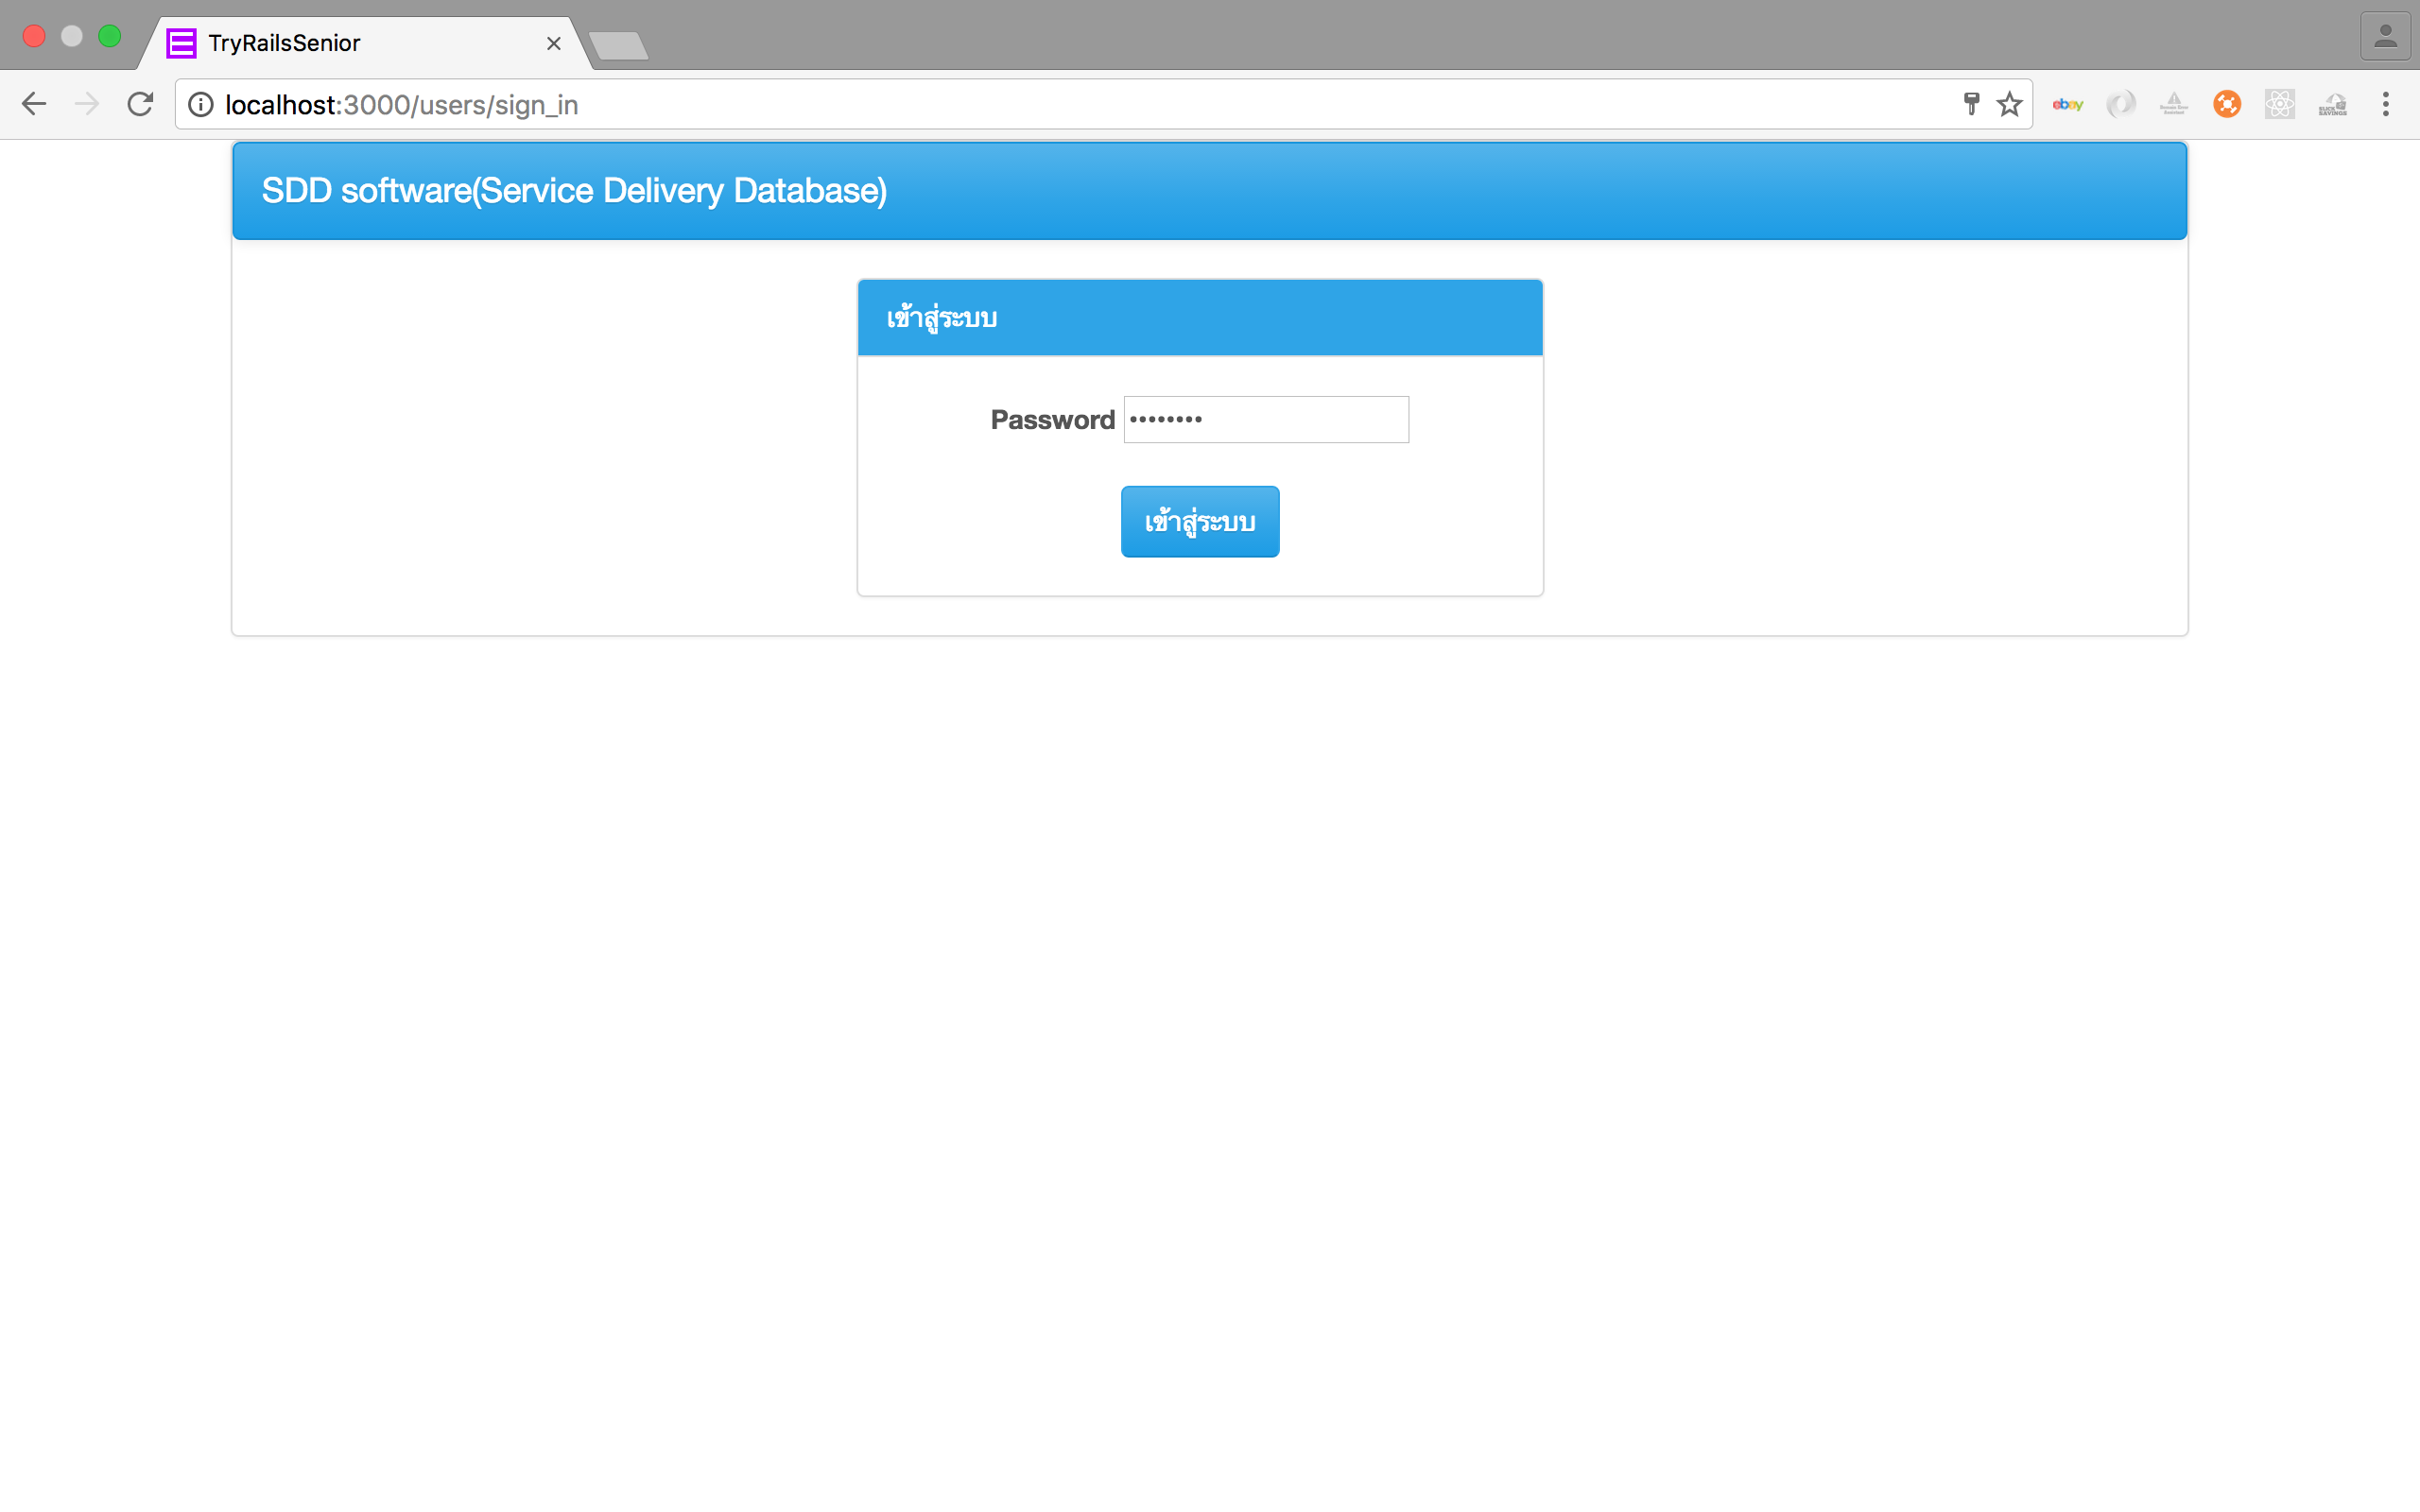
\includegraphics[width=12cm]{images/chapter-01/mockup_rails/log_in.png}
                    	\caption{Log-In Page}
                    	\label{log_in}
                \end{figure}
            \FloatBarrier
            
            \FloatBarrier
                \begin{figure}[h!]
                    \centering
                        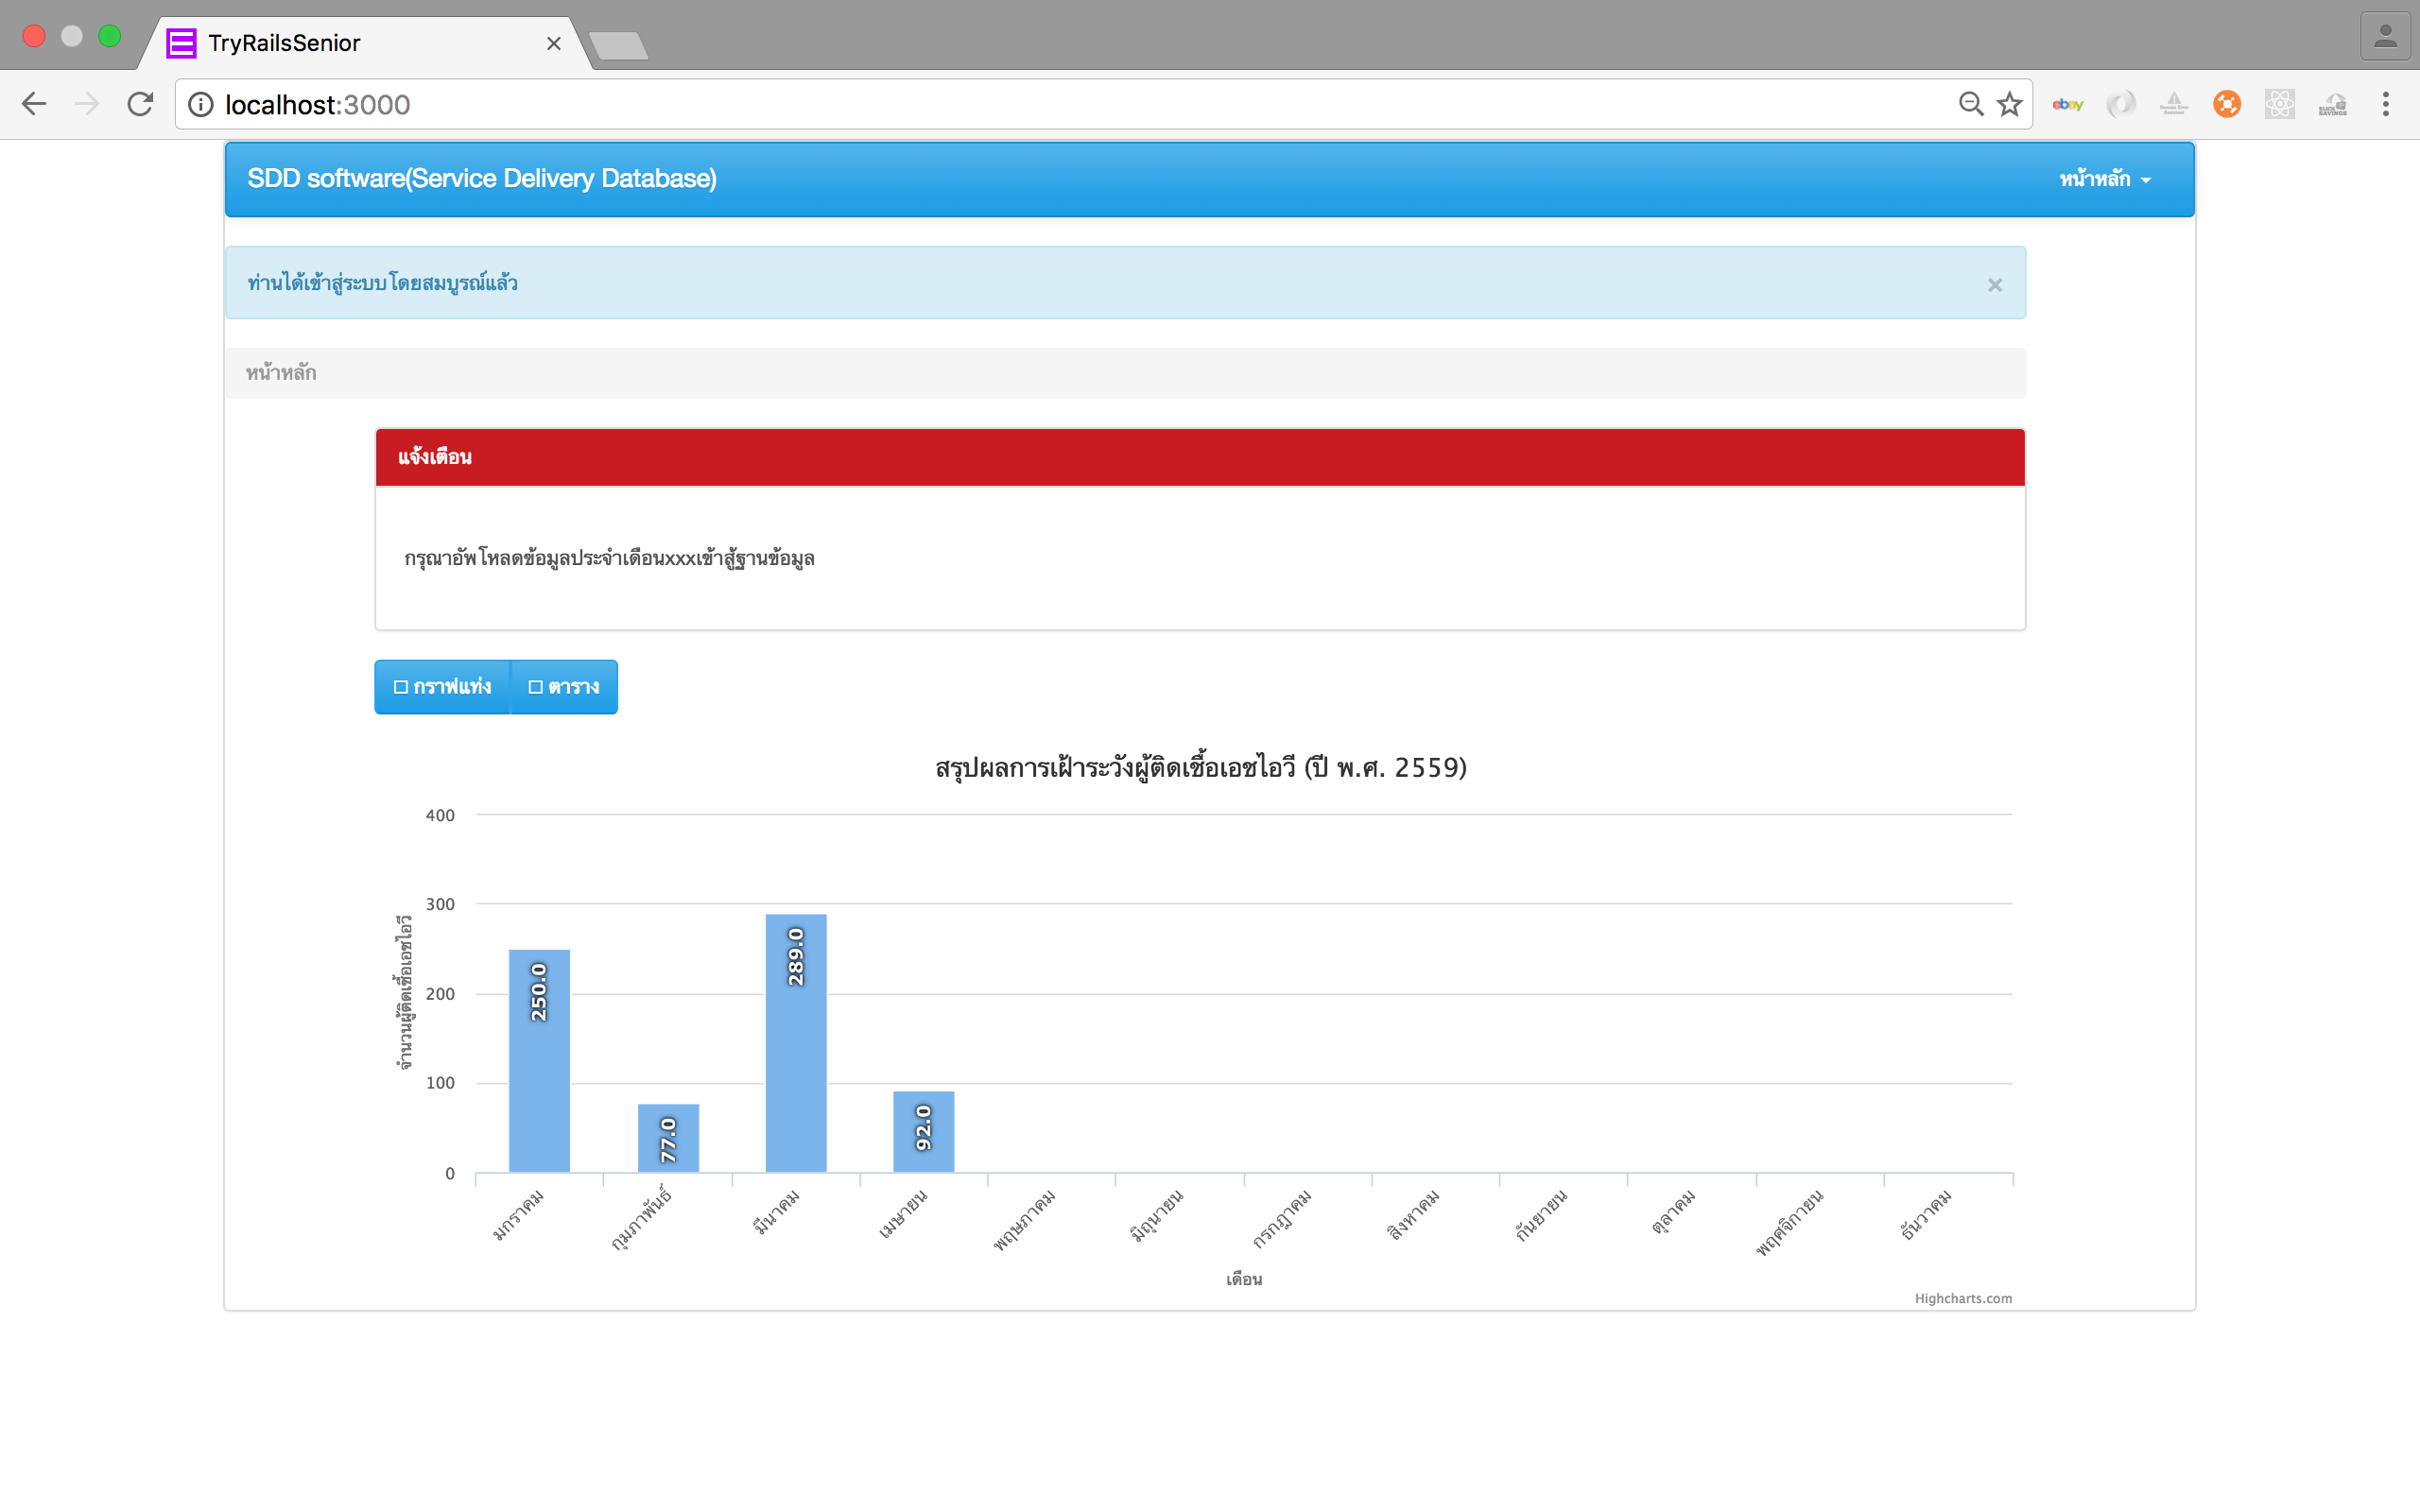
\includegraphics[width=12cm]{images/chapter-01/mockup_rails/home.png}
                    	\caption{Home Page}
                    	\label{home}
                \end{figure}
            \FloatBarrier
            
            \FloatBarrier
                \begin{figure}[h!]
                    \centering
                        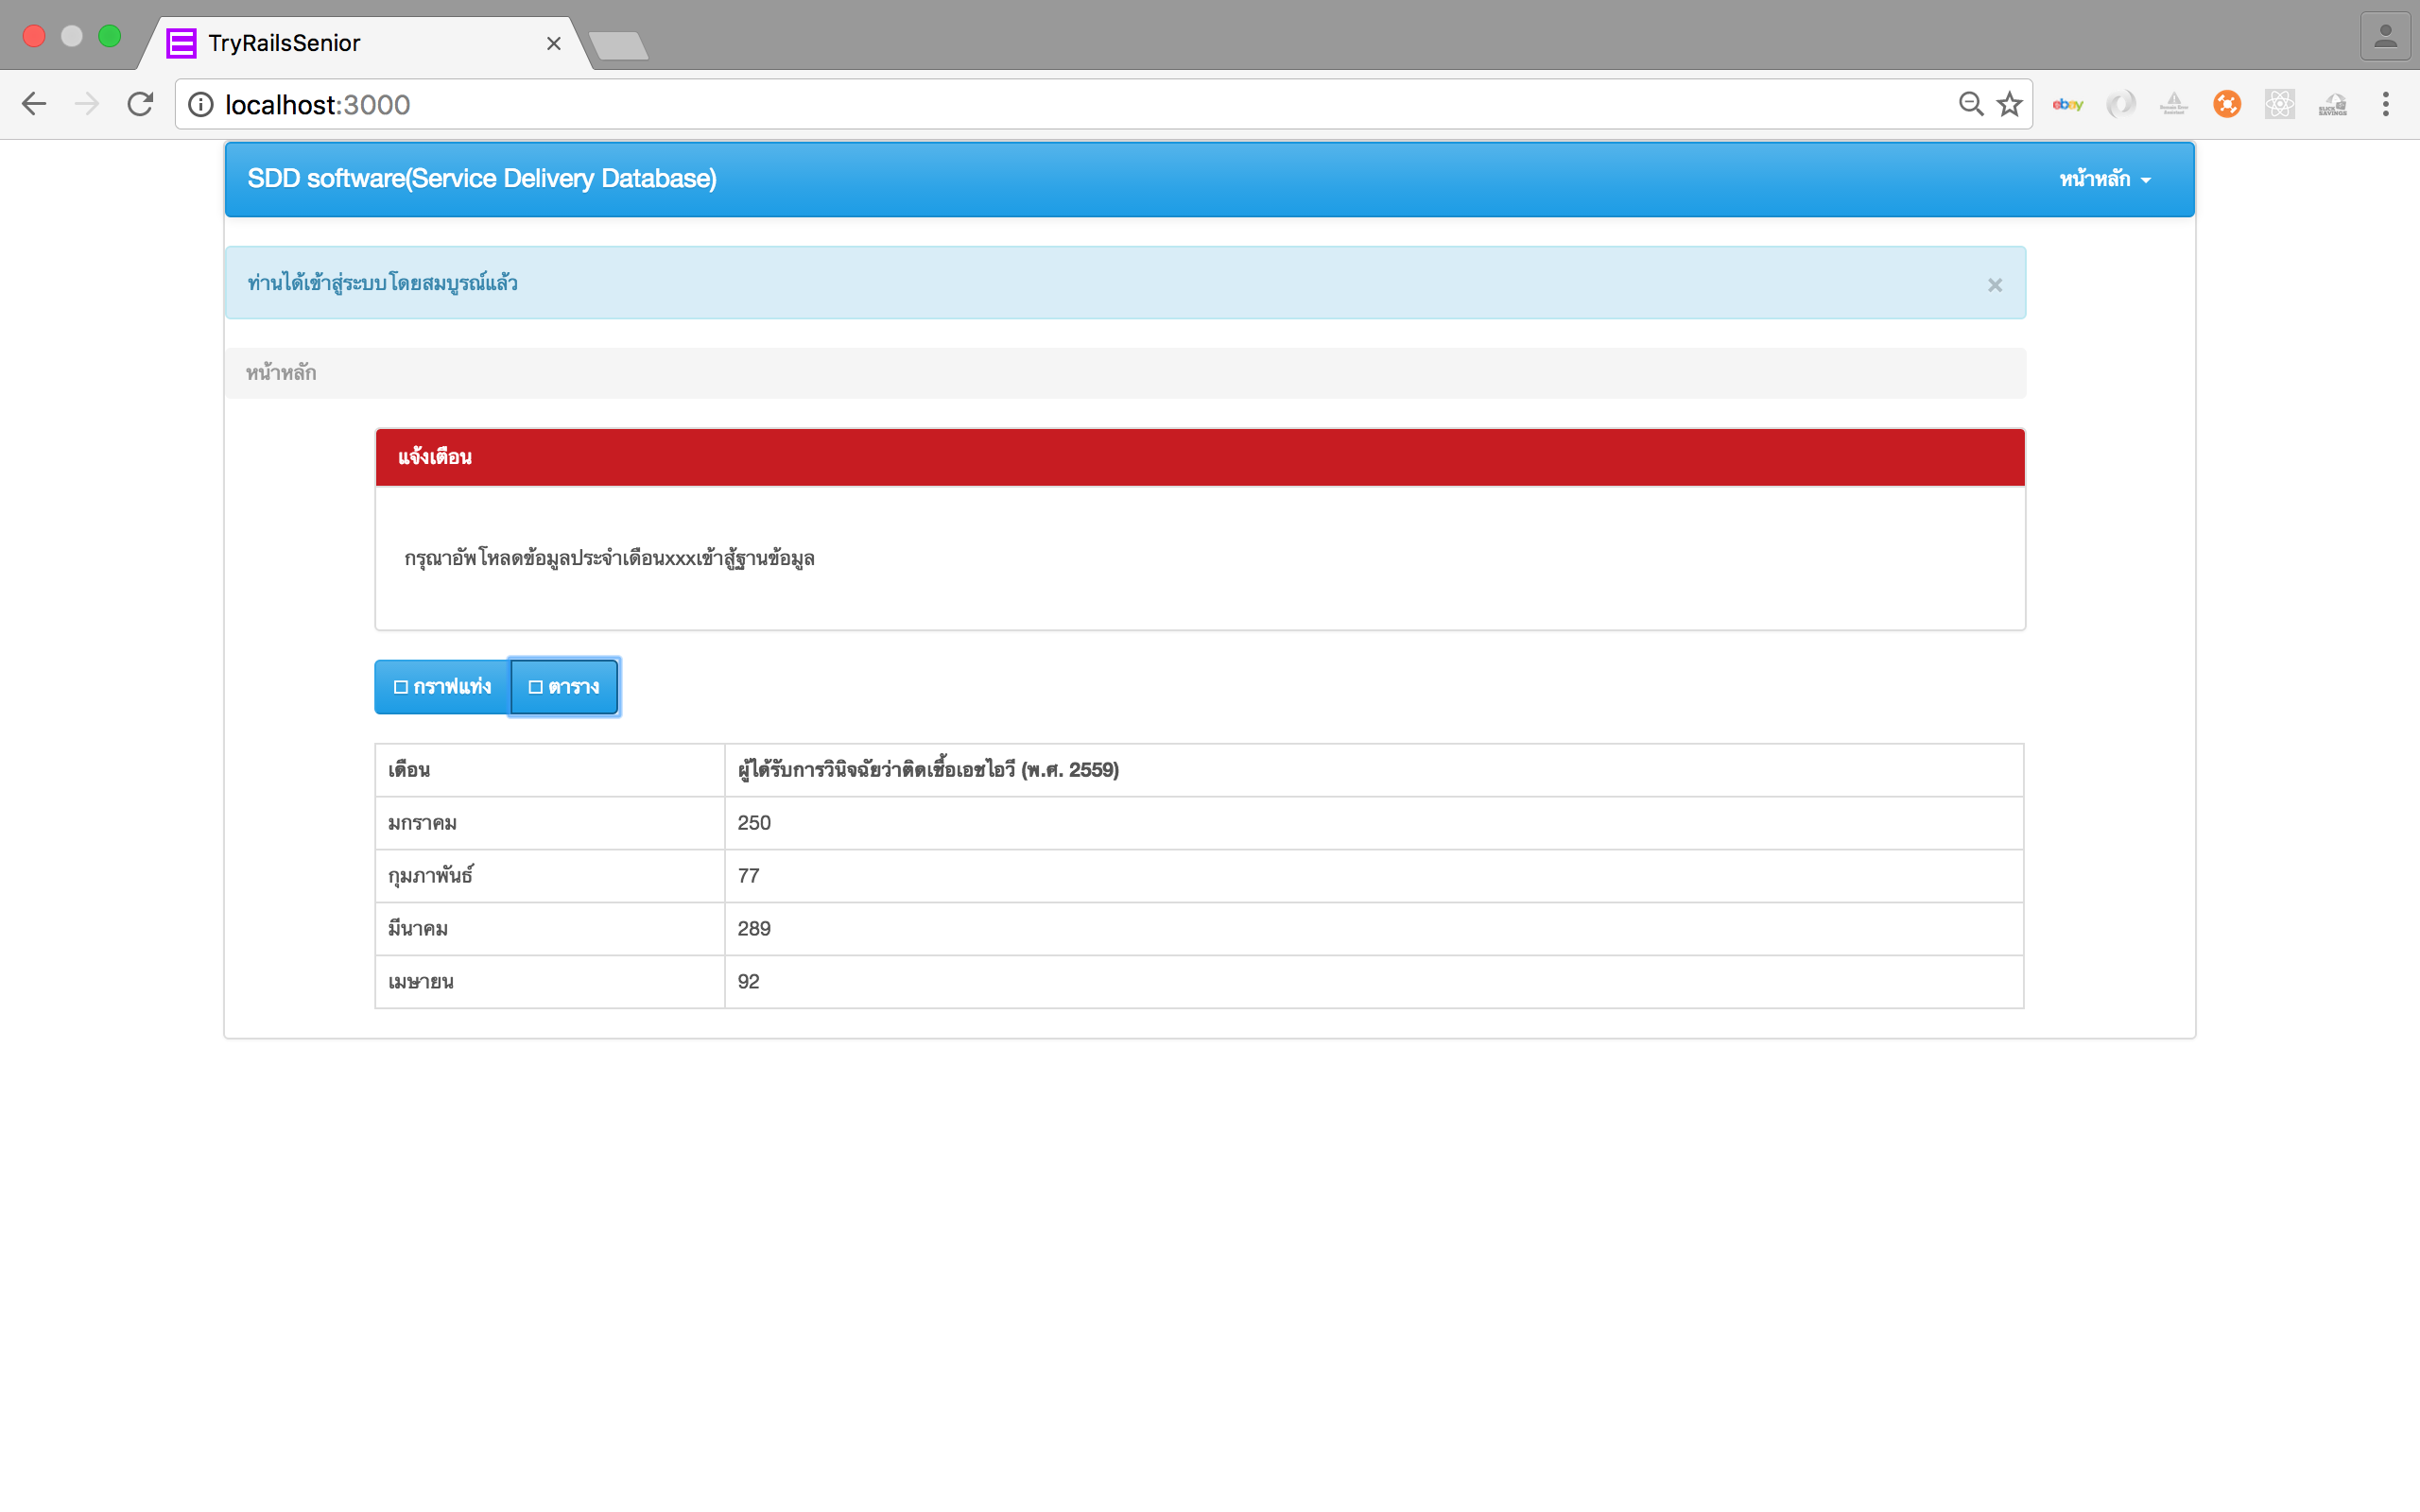
\includegraphics[width=12cm]{images/chapter-01/mockup_rails/home2.png}
                    	\caption{Home Page2}
                    	\label{home2}
                \end{figure}
            \FloatBarrier
        
            \FloatBarrier
                \begin{figure}[h!]
                    \centering
                        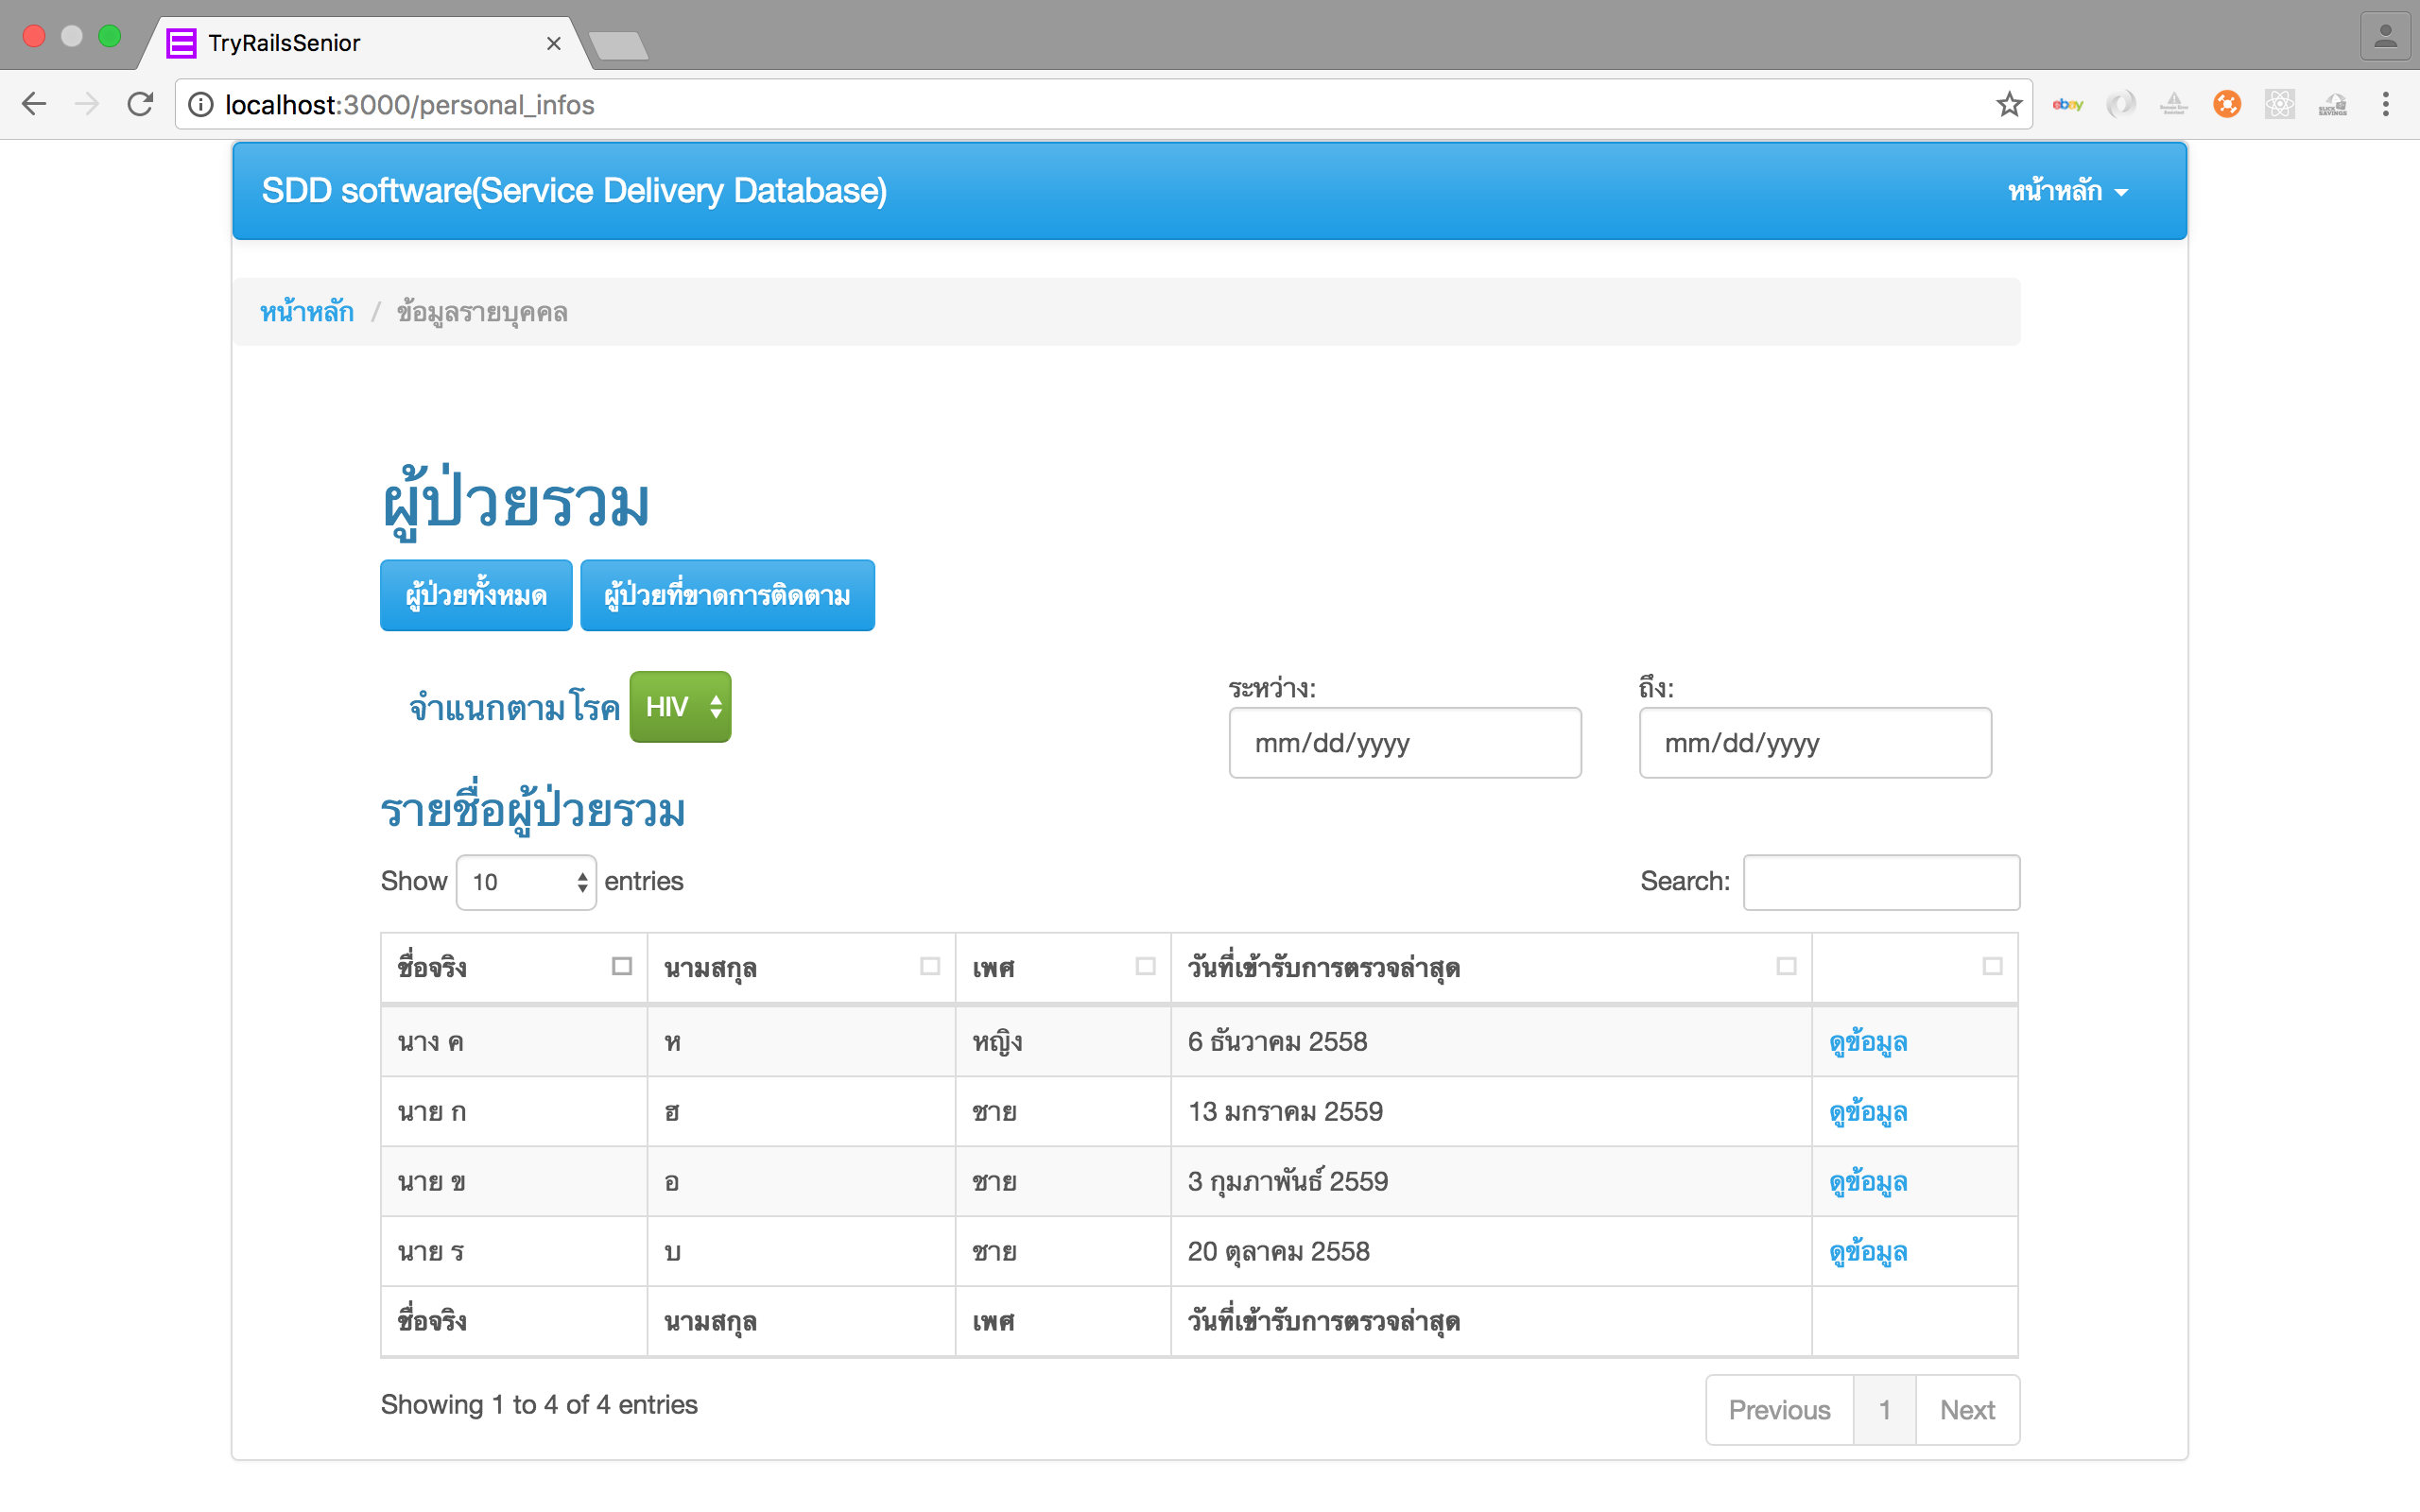
\includegraphics[width=12cm]{images/chapter-01/mockup_rails/individual_report.png}
                    	\caption{Individual Report Table}
                    	\label{individual_report}
                \end{figure}
            \FloatBarrier
            \FloatBarrier
                \begin{figure}[h!]
                    \centering
                        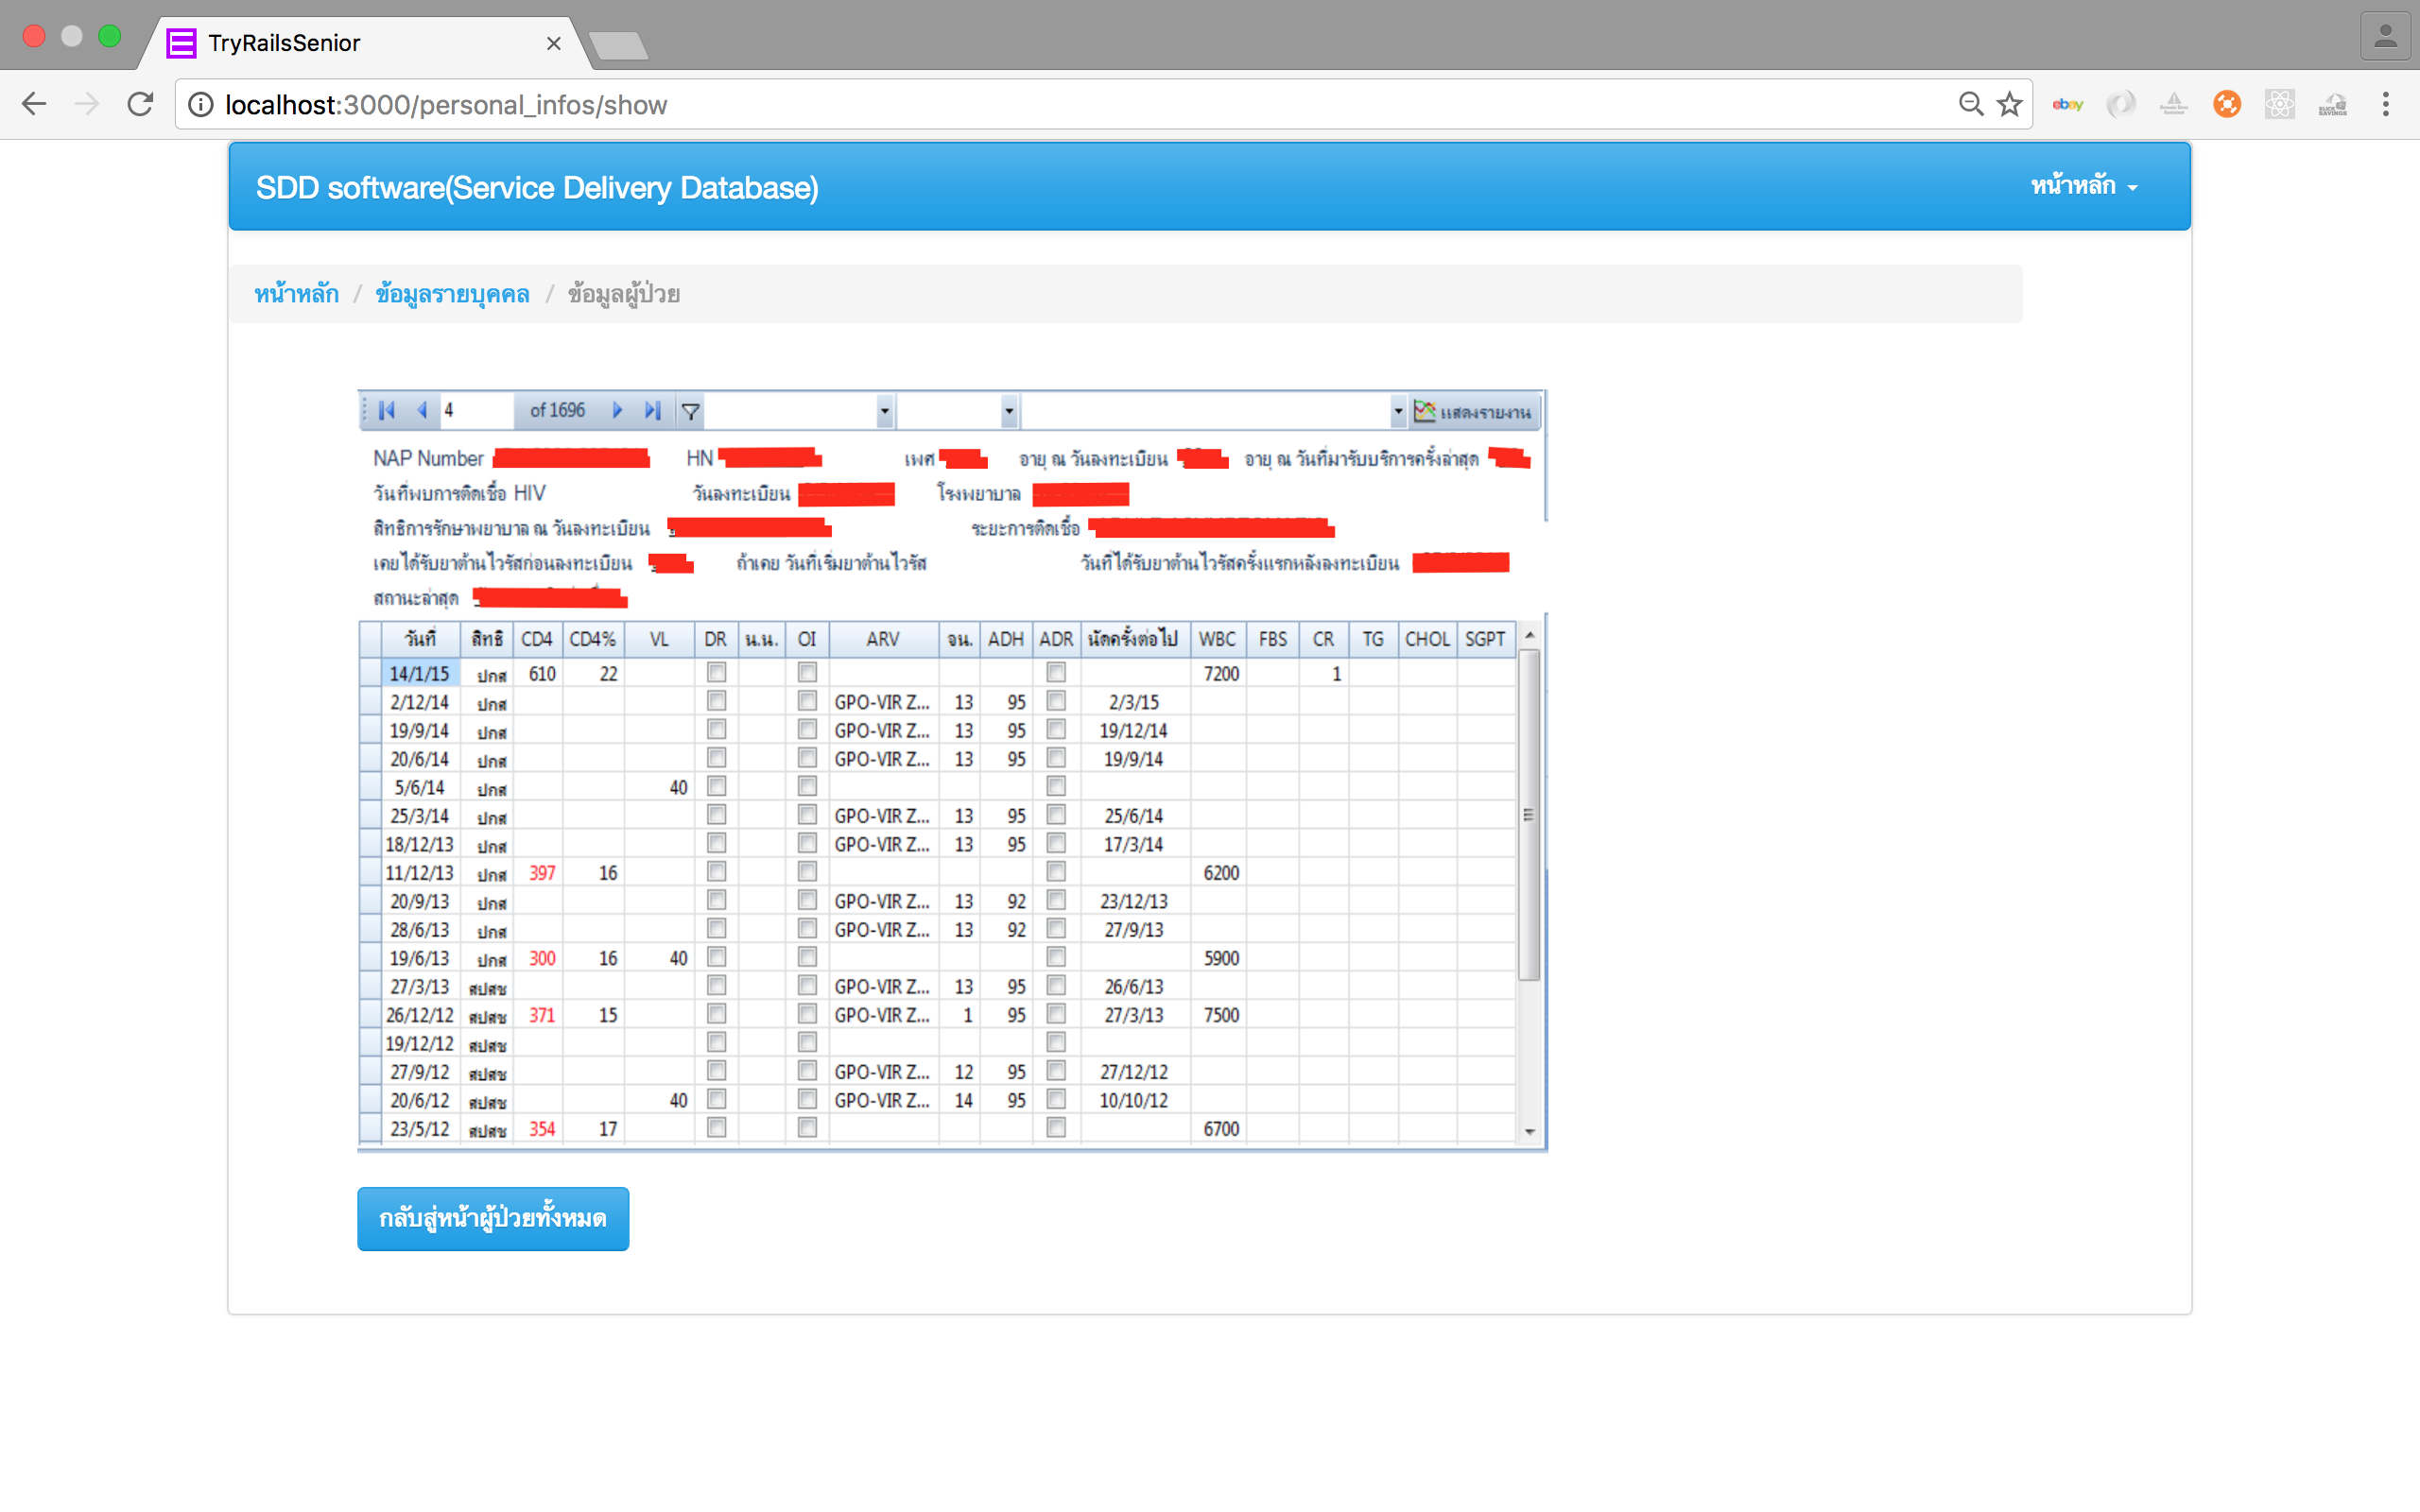
\includegraphics[width=12cm]{images/chapter-01/mockup_rails/individual_report1.png}
                    	\caption{Individual Report Details}
                    	\label{individual_report1}
                \end{figure}
            \FloatBarrier
            
            \FloatBarrier
                \begin{figure}[h!]
                    \centering
                        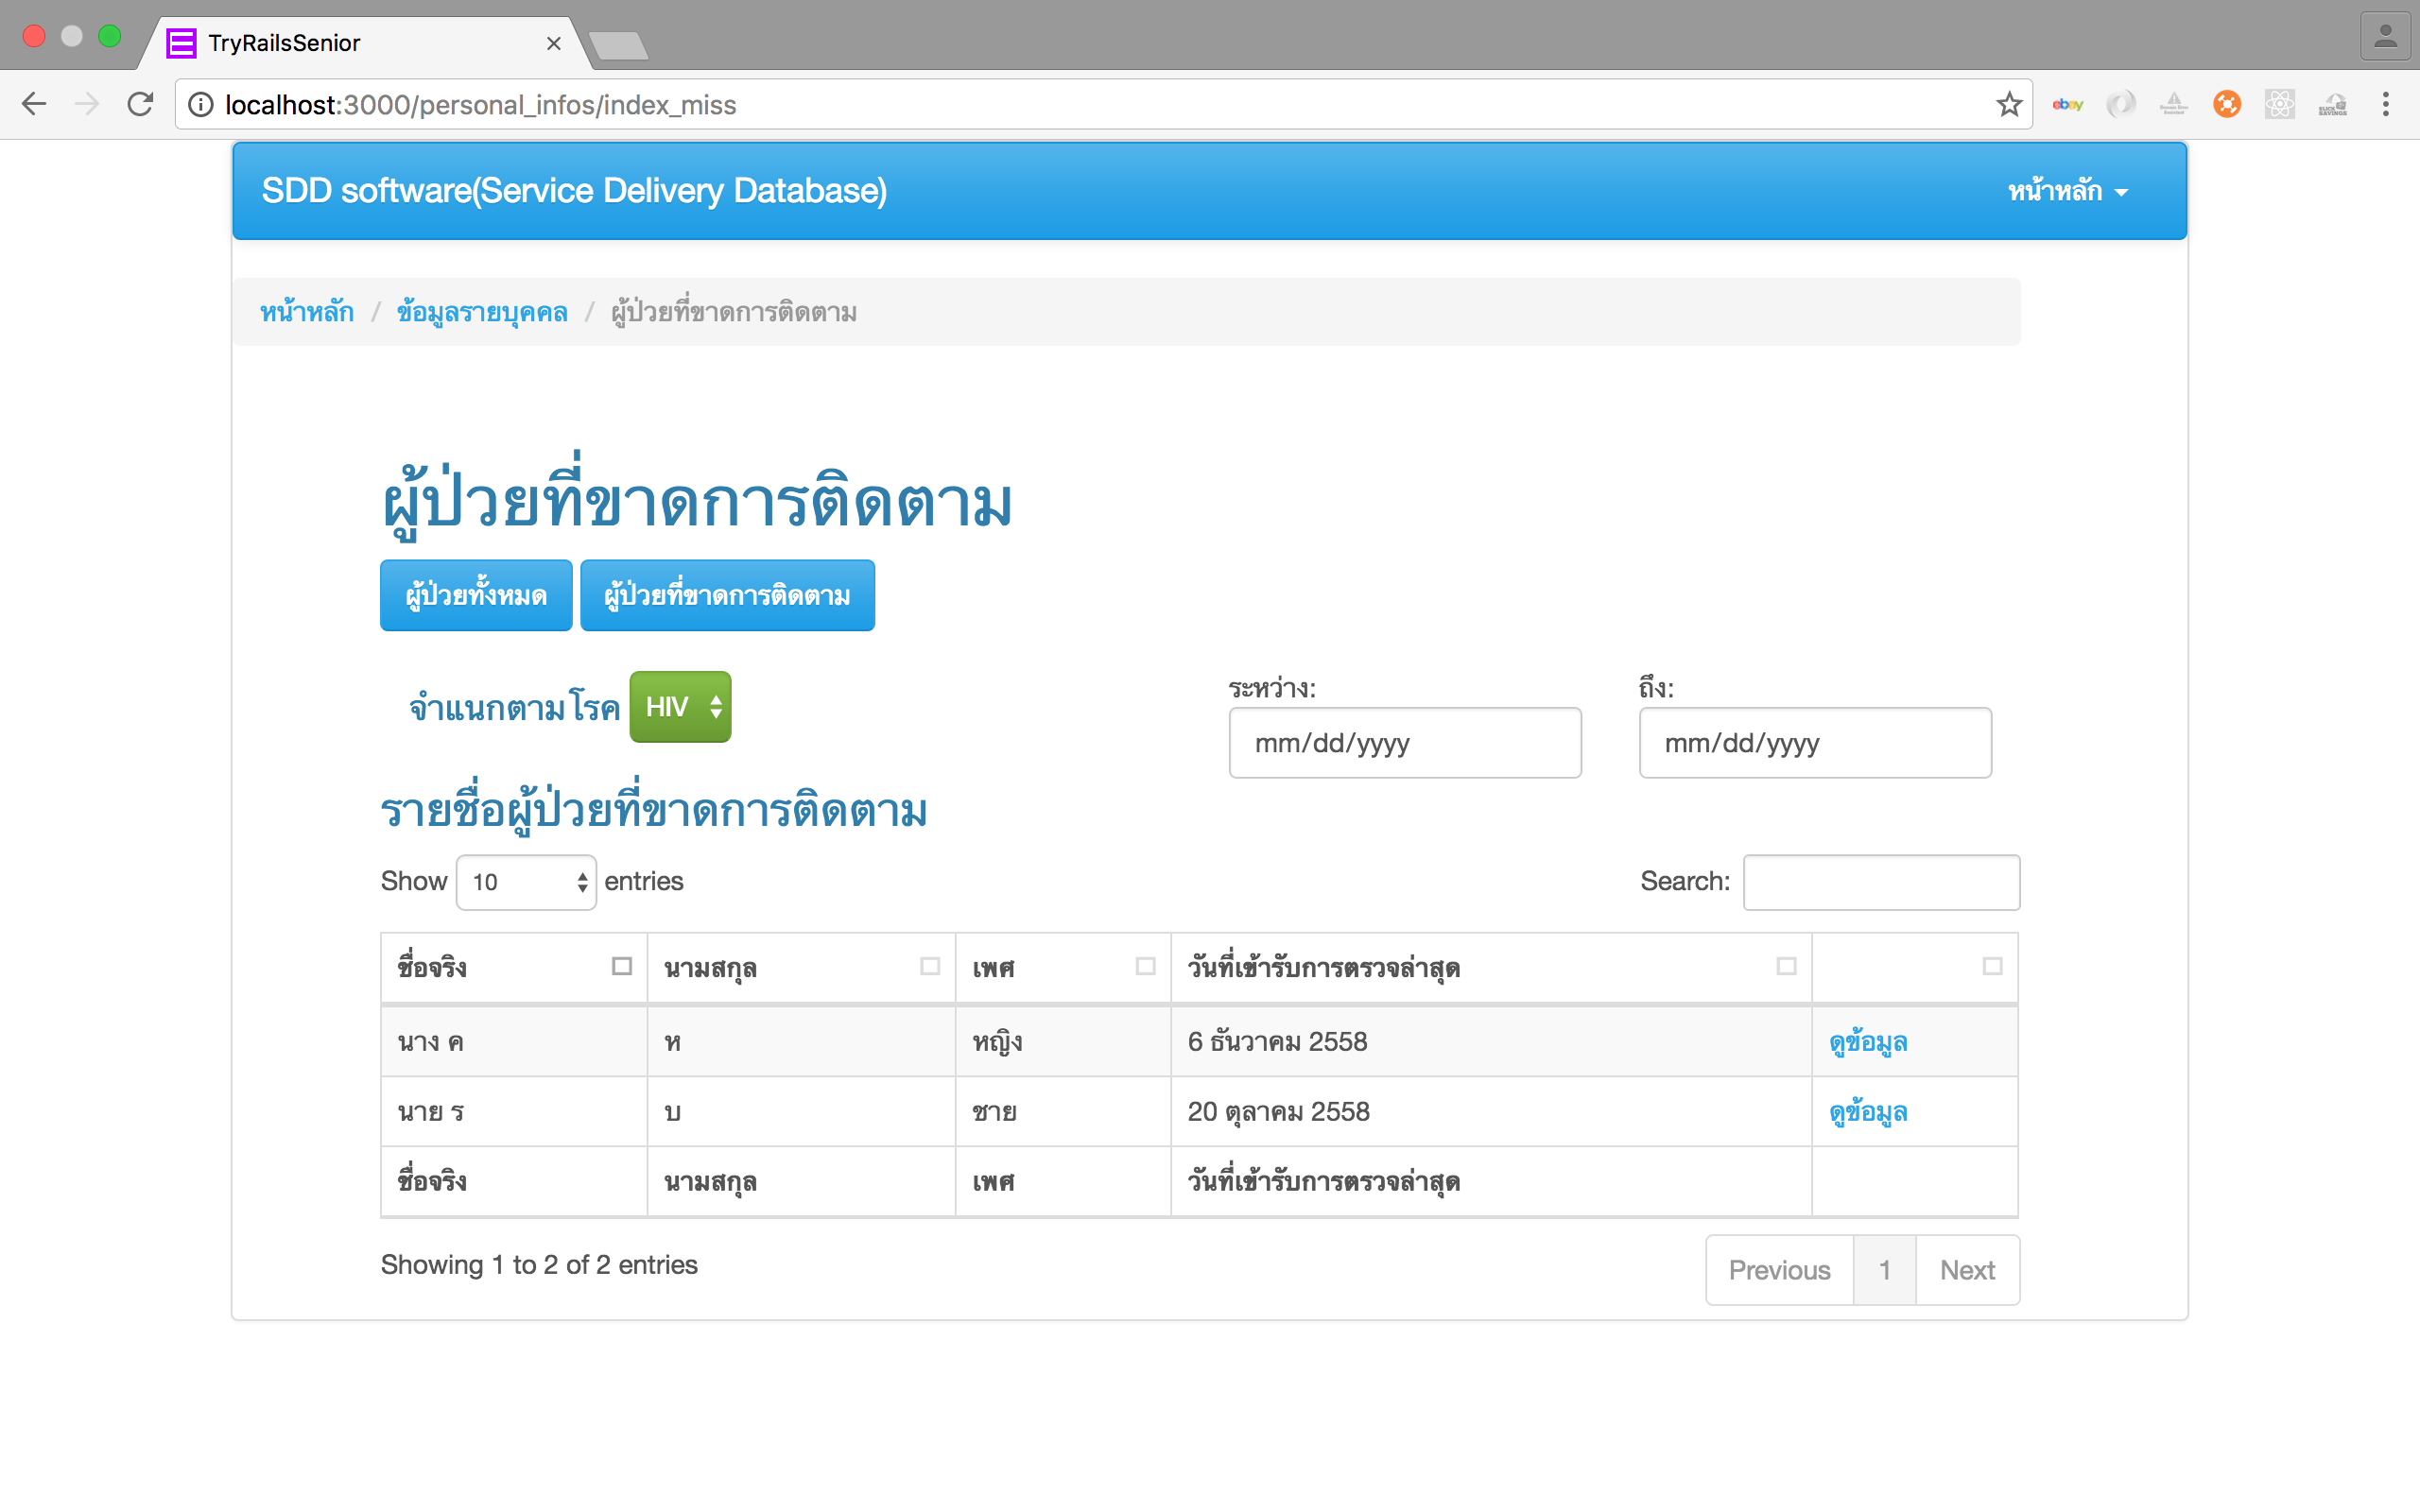
\includegraphics[width=12cm]{images/chapter-01/mockup_rails/lost_follow_up.png}
                    	\caption{Lost Follow Table}
                    	\label{lost_follow_up}
                \end{figure}
            \FloatBarrier
            
            \FloatBarrier
                \begin{figure}[h!]
                    \centering
                        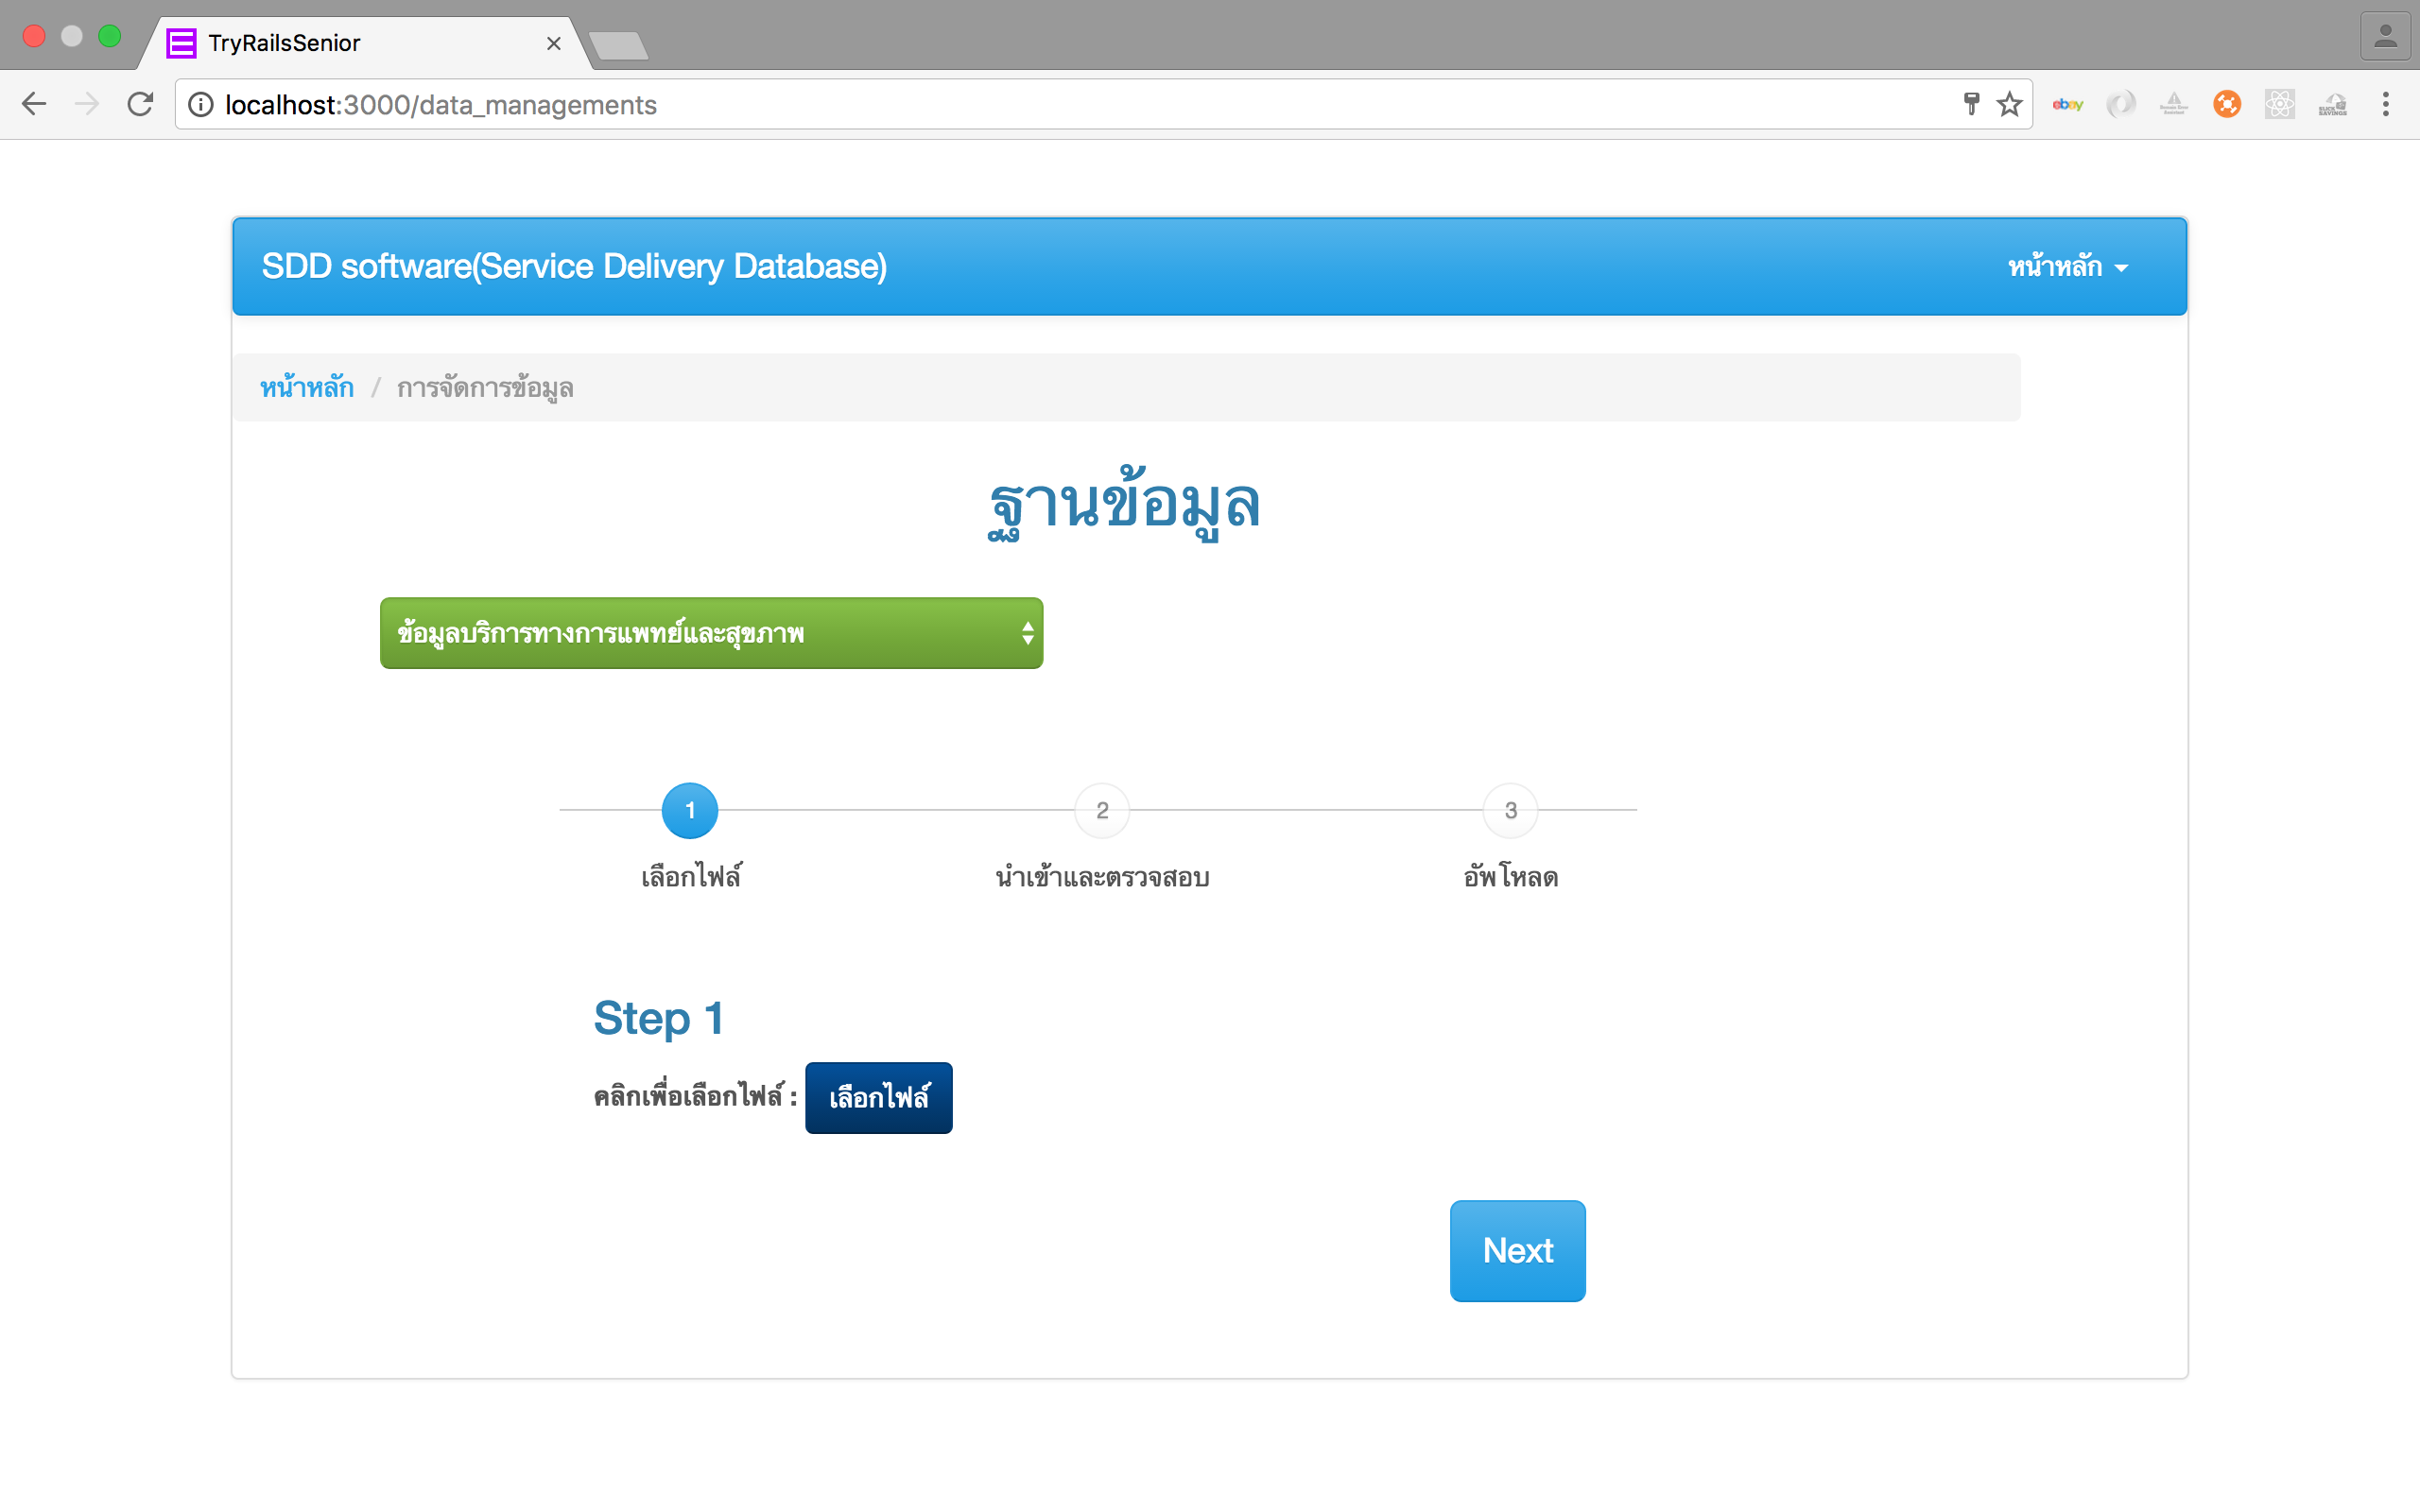
\includegraphics[width=12cm]{images/chapter-01/mockup_rails/upload.png}
                    	\caption{Upload Page Status 1}
                    	\label{upload}
                \end{figure}
            \FloatBarrier
            
           \FloatBarrier
                \begin{figure}[h!]
                    \centering
                        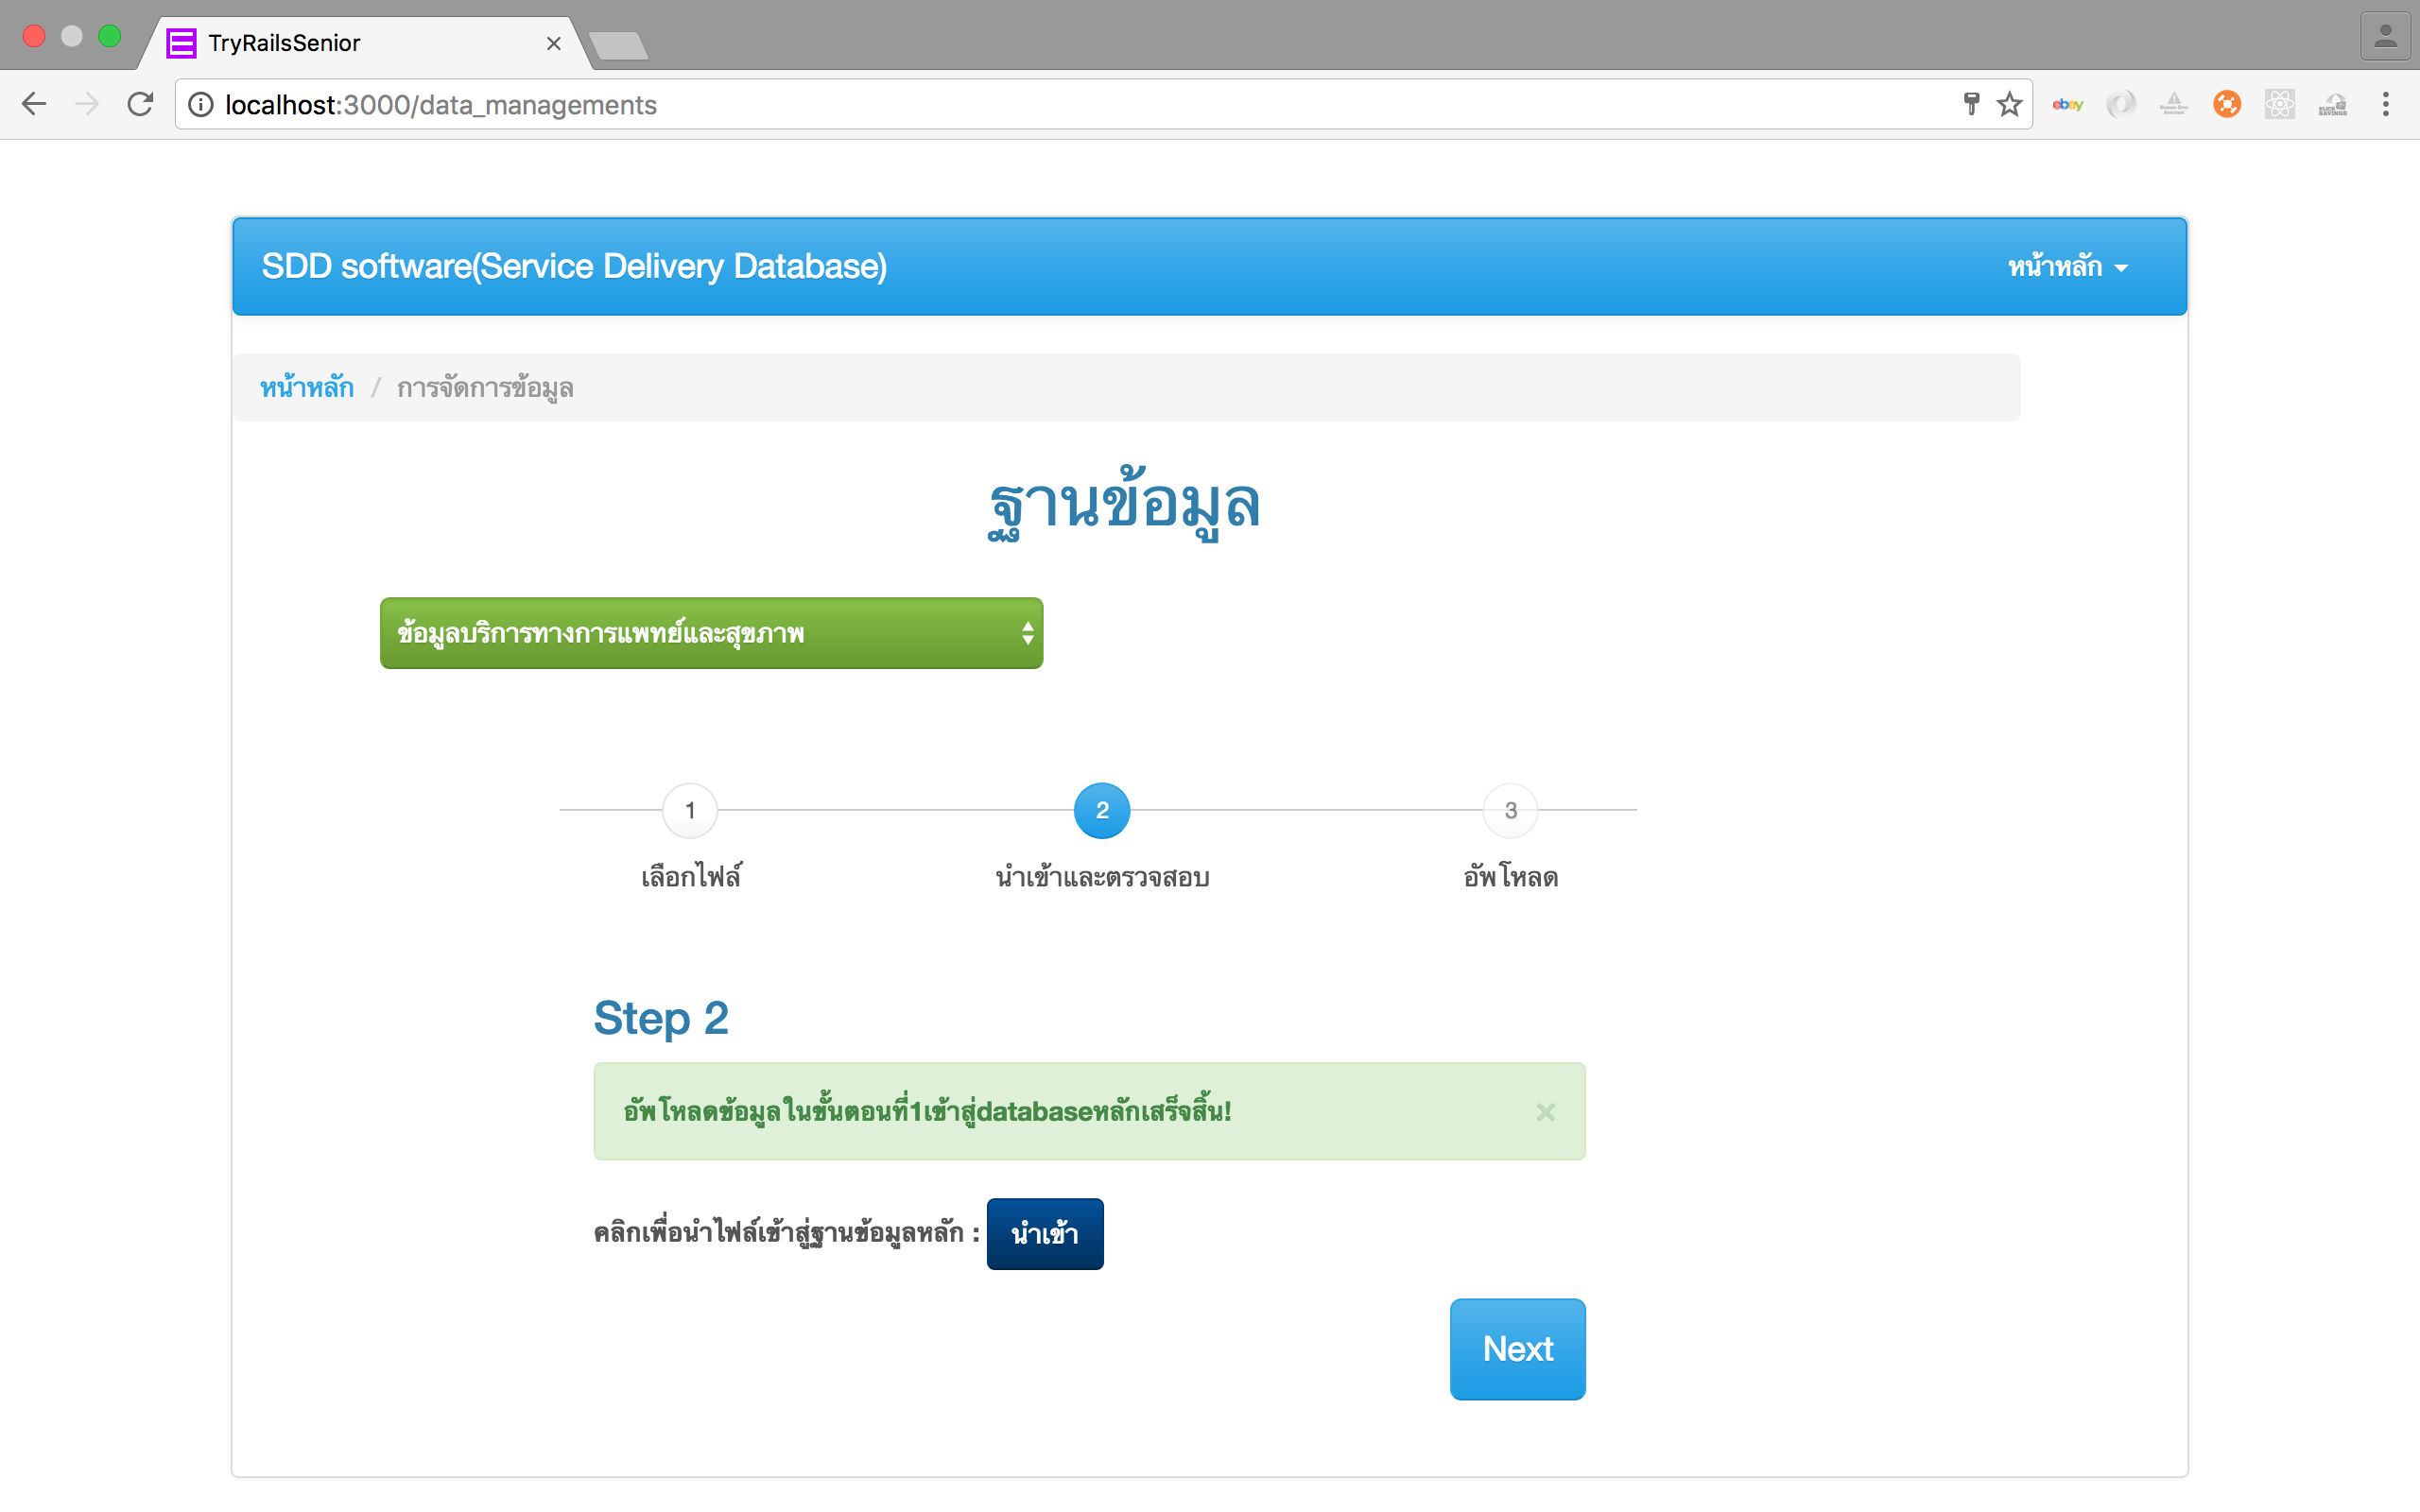
\includegraphics[width=12cm]{images/chapter-01/mockup_rails/upload2.png}
                    	\caption{Upload Page Status 2}
                    	\label{upload2}
                \end{figure}
            \FloatBarrier
            
            \FloatBarrier
                \begin{figure}[h!]
                    \centering
                        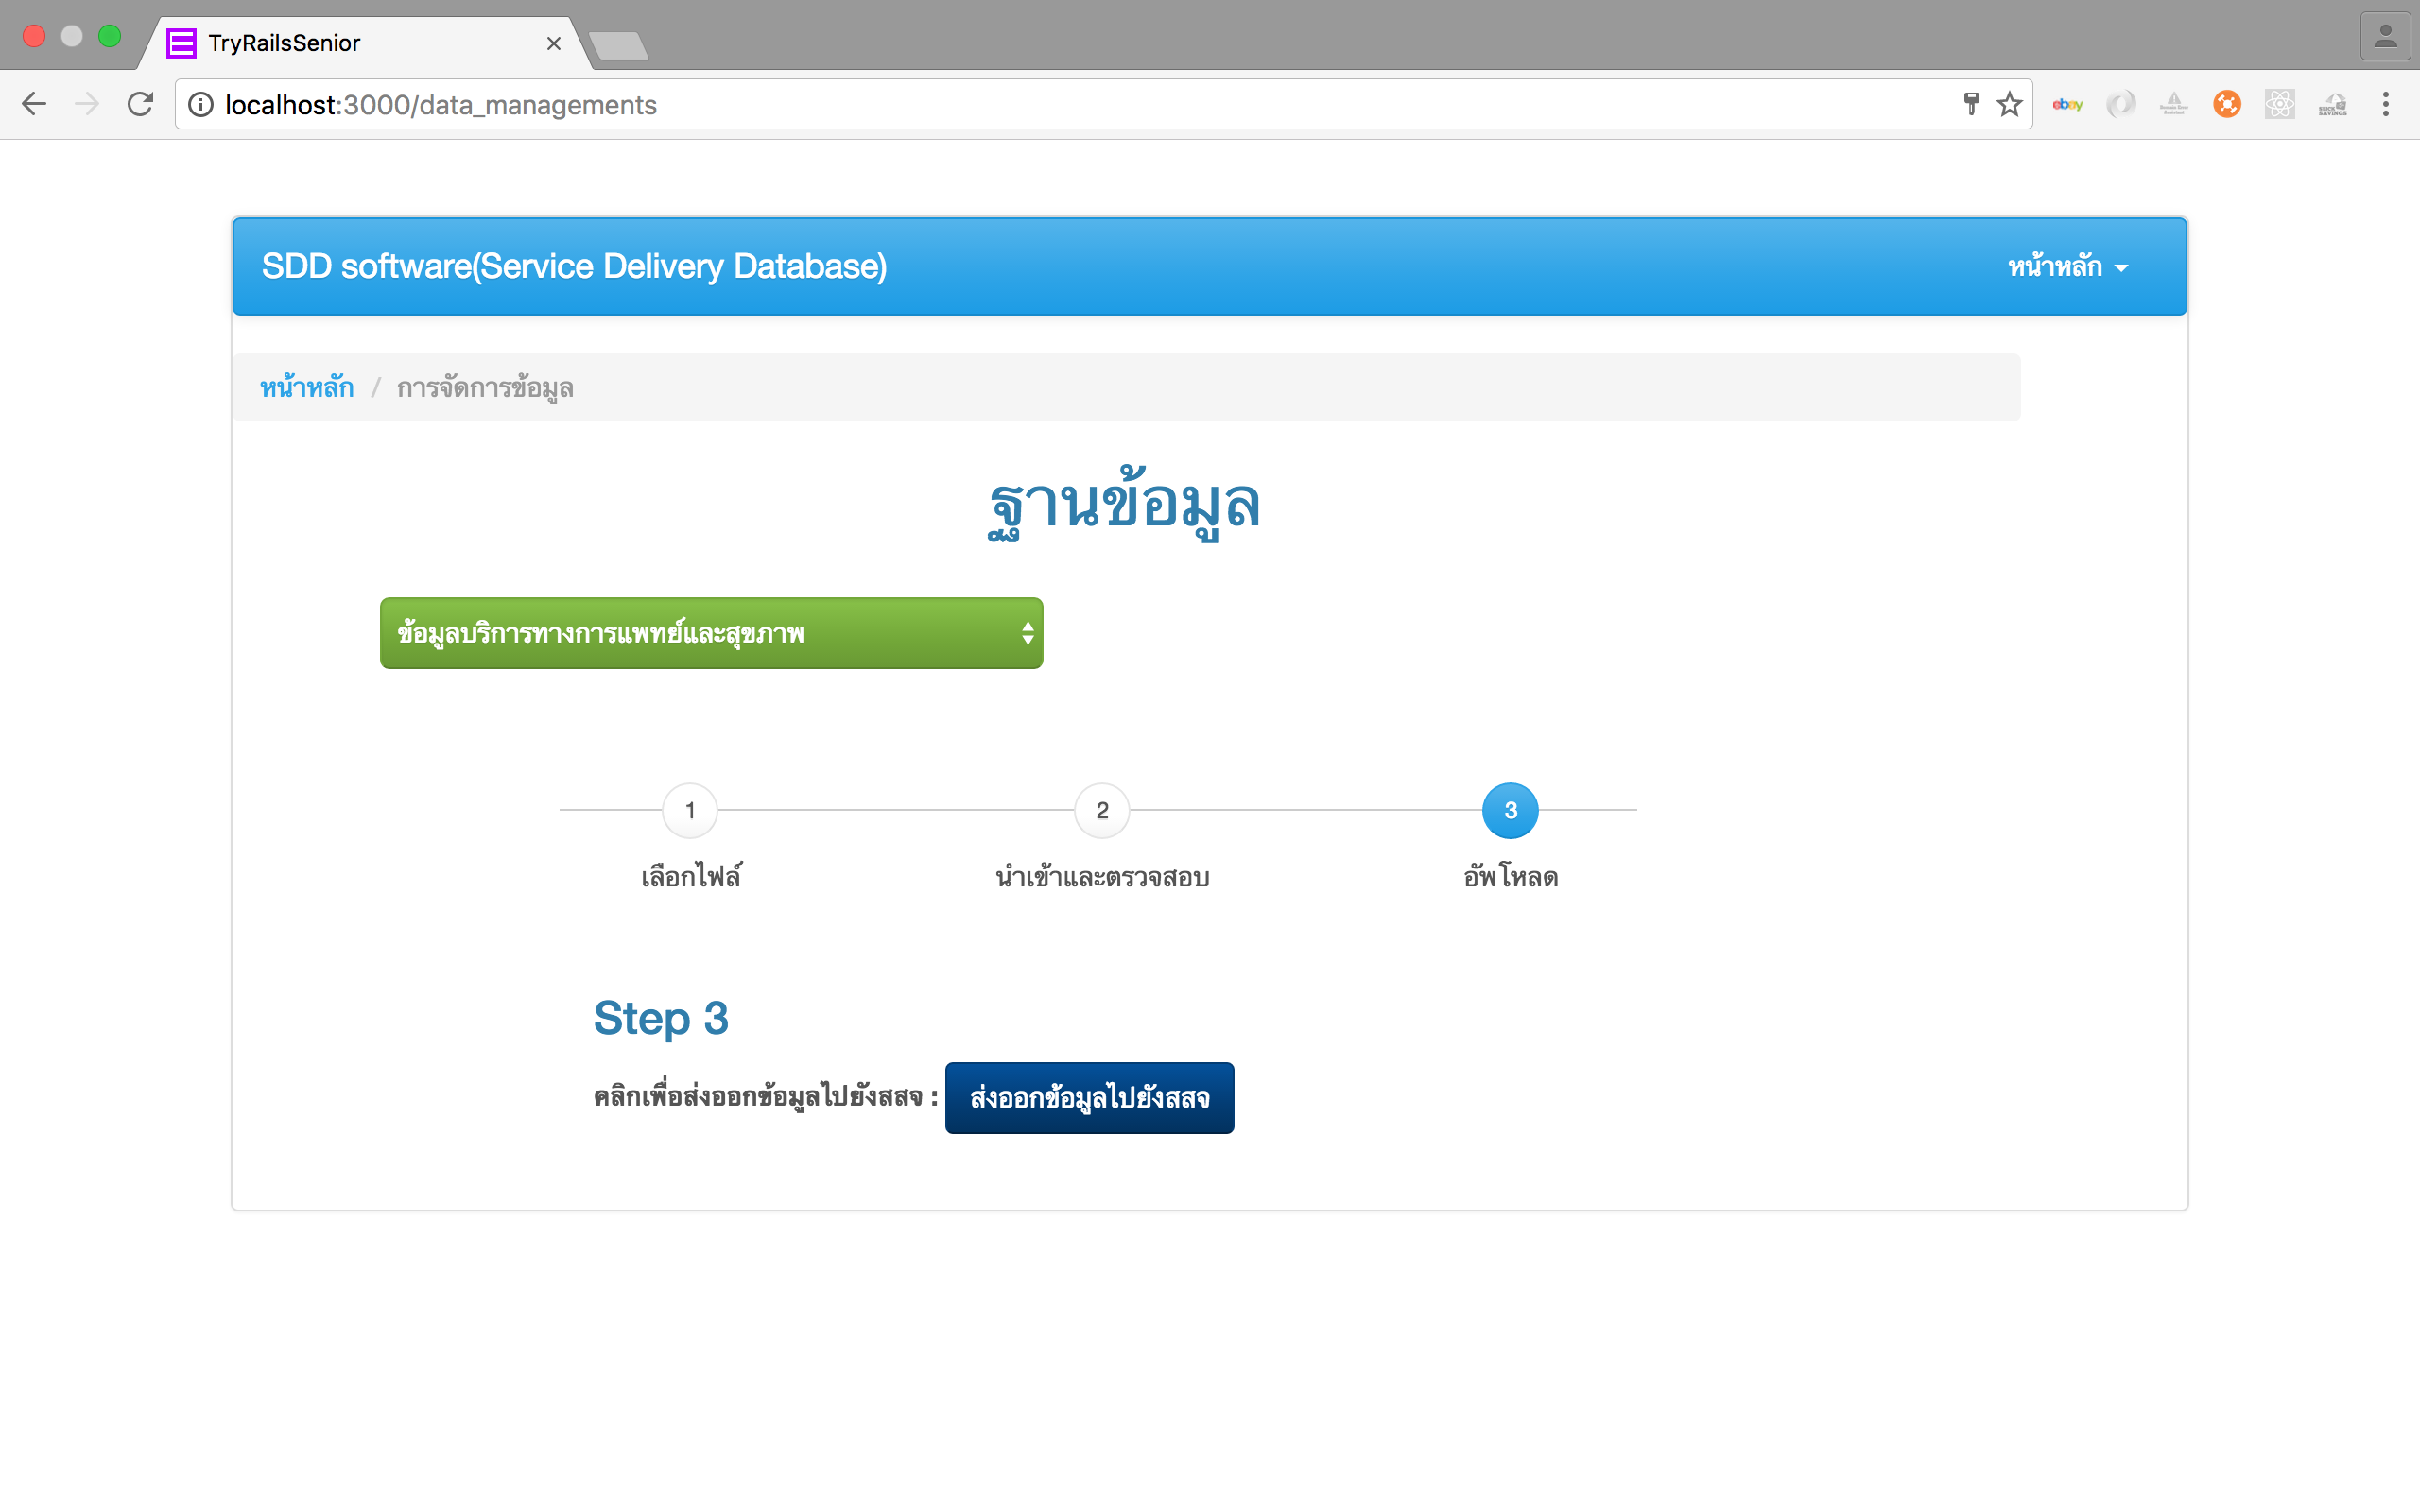
\includegraphics[width=12cm]{images/chapter-01/mockup_rails/upload3.png}
                    	\caption{Upload Page Status 3}
                    	\label{upload3}
                \end{figure}
            \FloatBarrier
            
            \FloatBarrier
                \begin{figure}[h!]
                    \centering
                        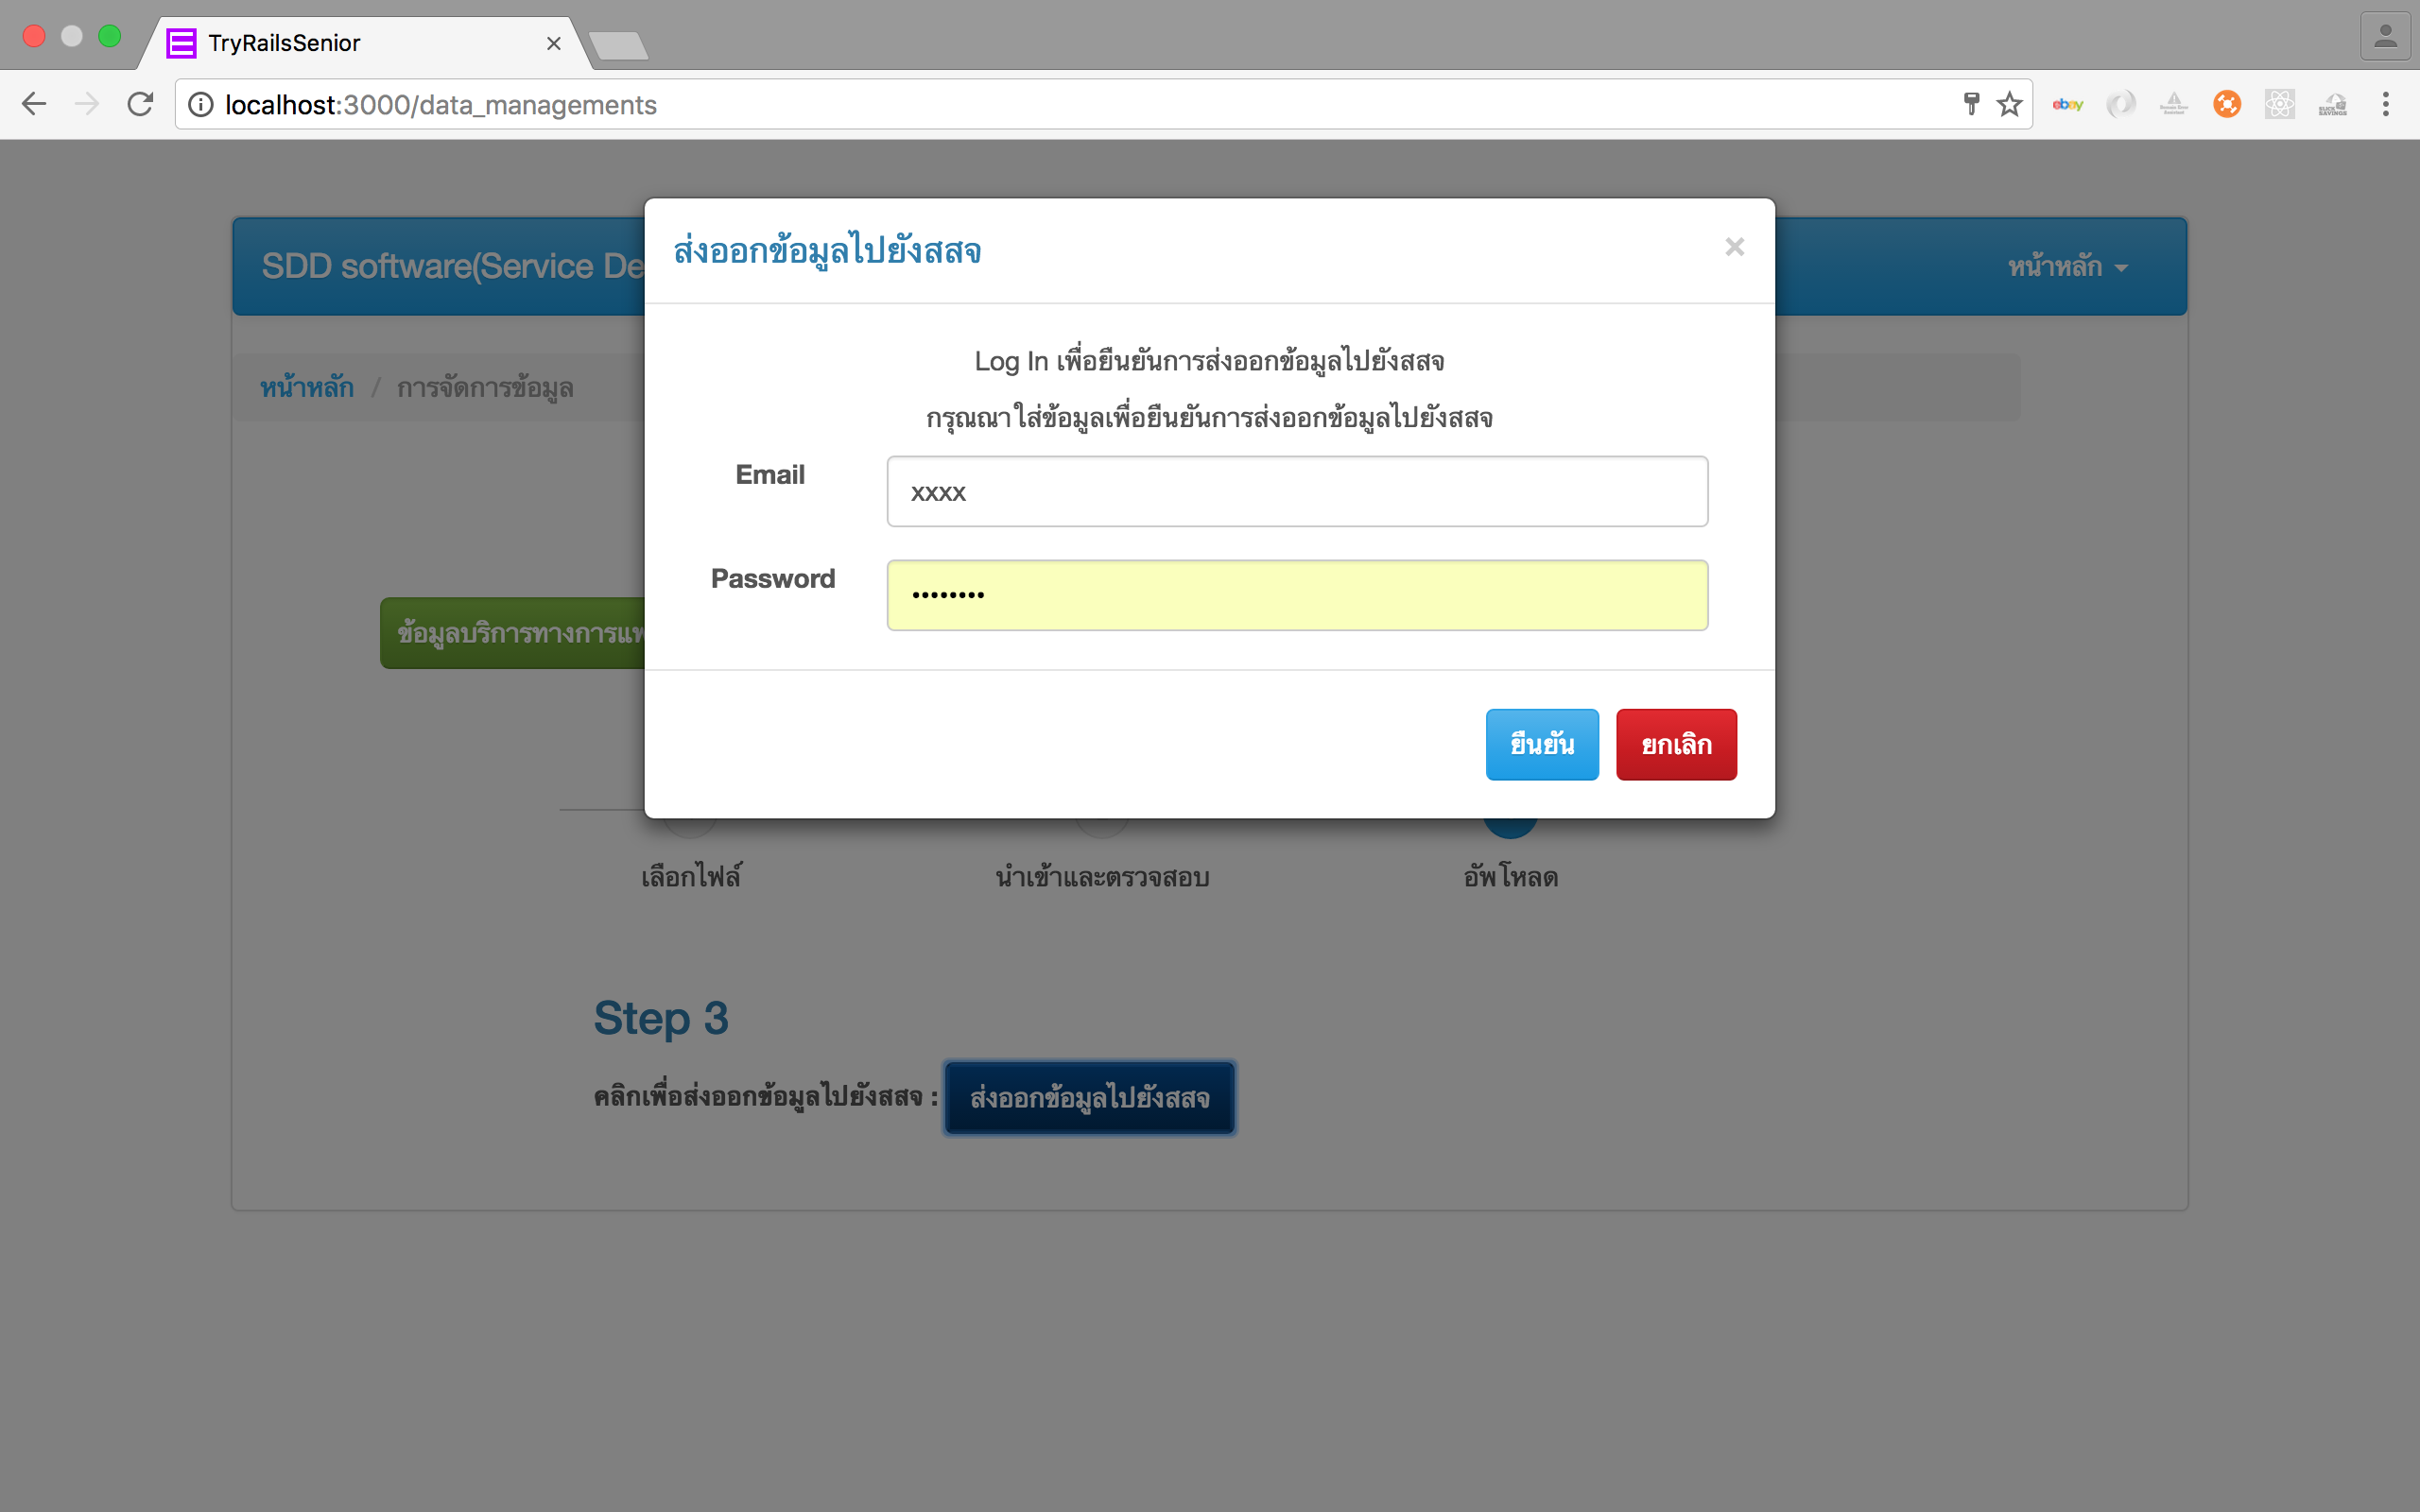
\includegraphics[width=12cm]{images/chapter-01/mockup_rails/upload_confirm.png}
                    	\caption{Upload Confirm Pop Up}
                    	\label{upload_confirm}
                \end{figure}
            \FloatBarrier
            
            \FloatBarrier
                \begin{figure}[h!]
                    \centering
                        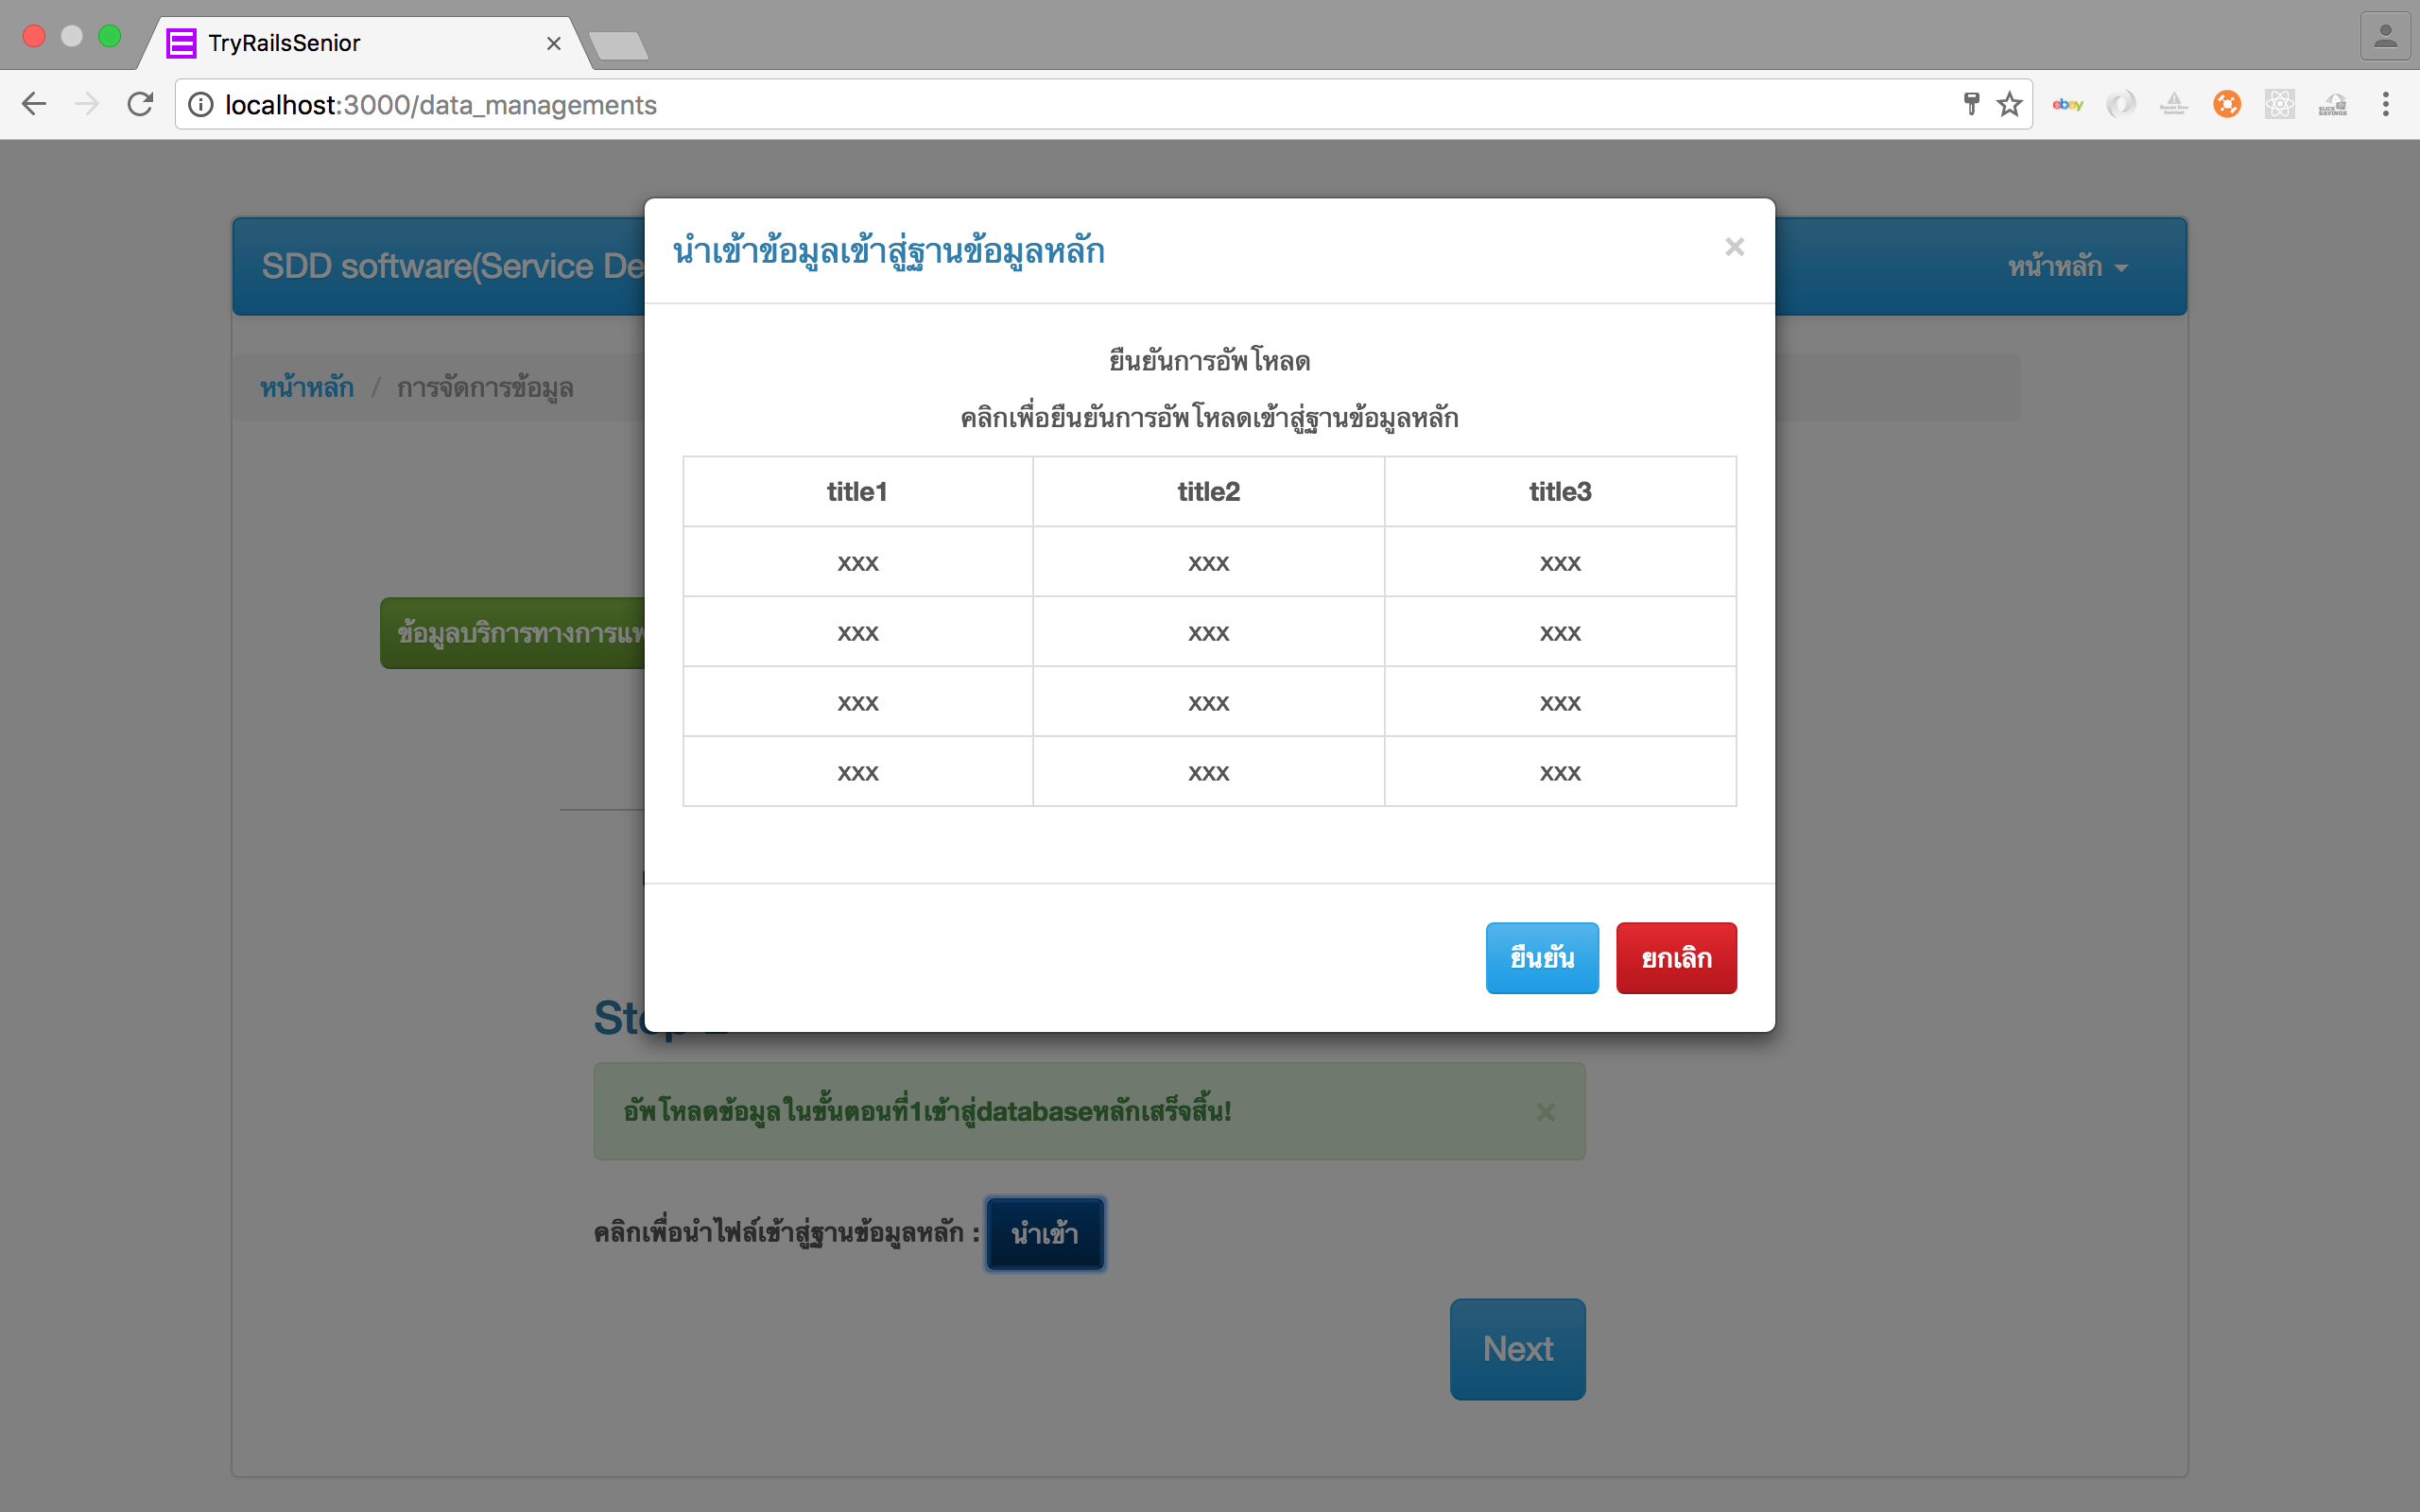
\includegraphics[width=12cm]{images/chapter-01/mockup_rails/upload_verify.png}
                    	\caption{Upload Verify Pop Up}
                    	\label{upload_verify}
                \end{figure}
            \FloatBarrier
            
            \FloatBarrier
                \begin{figure}[h!]
                    \centering
                        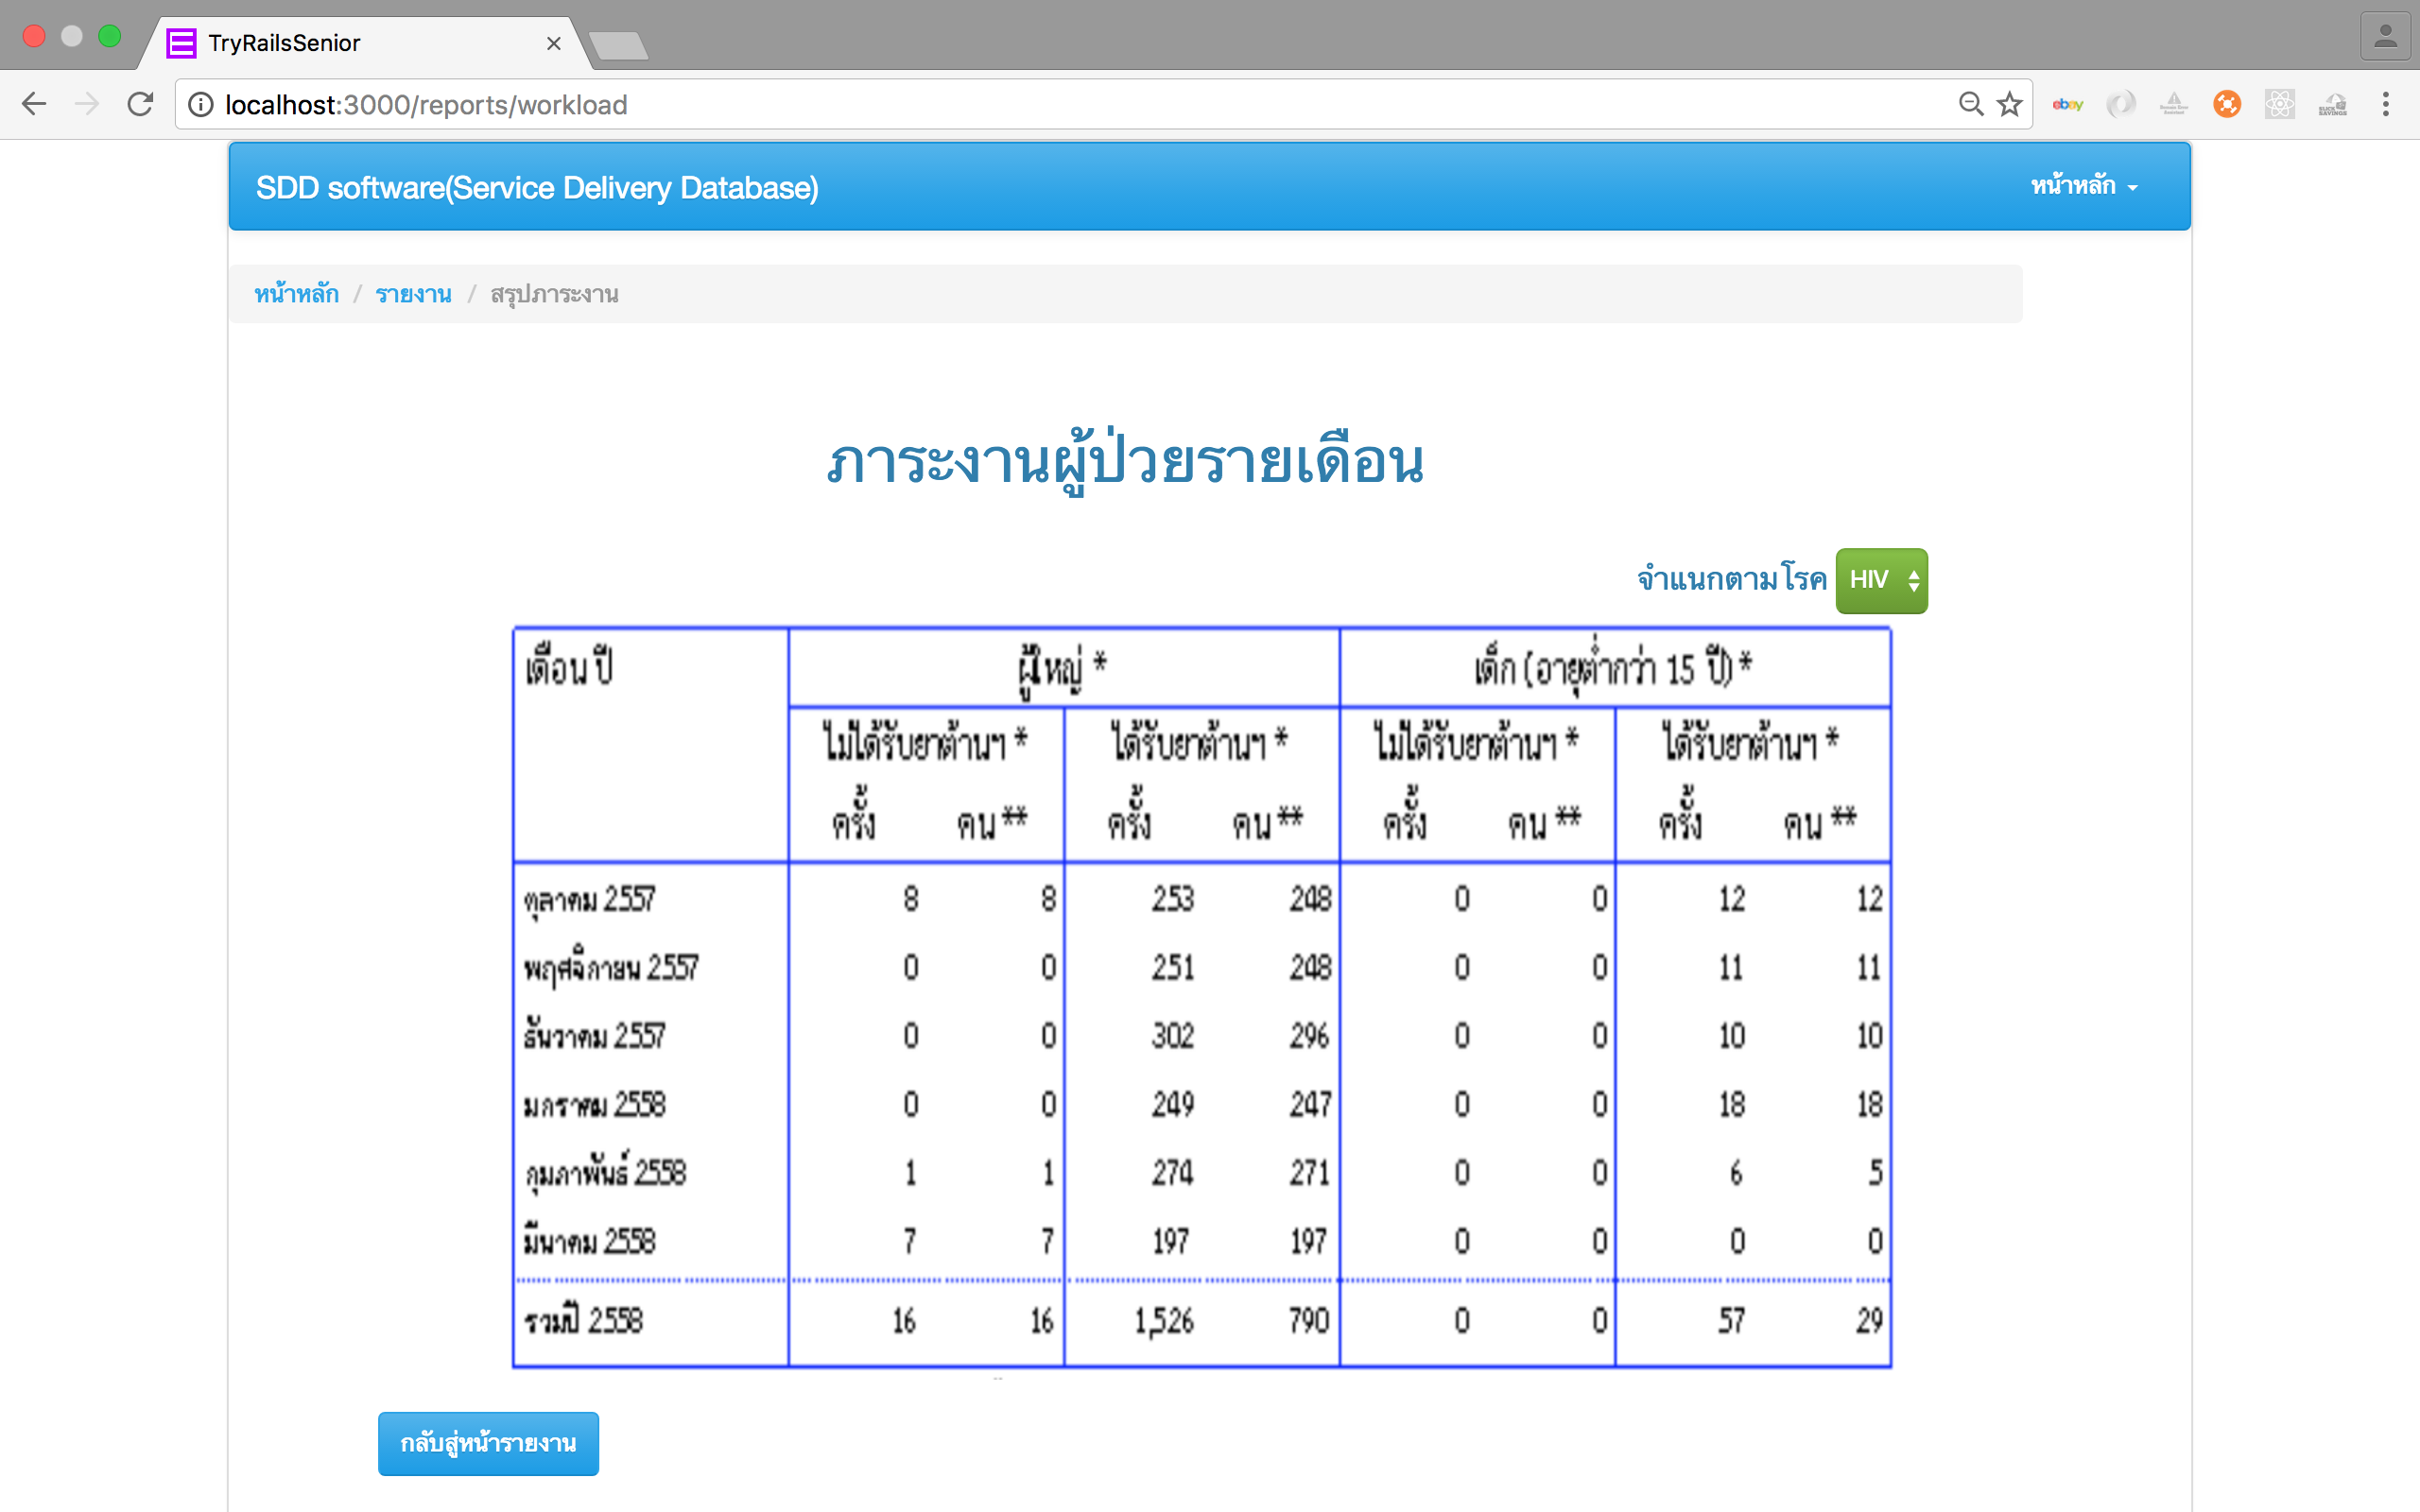
\includegraphics[width=12cm]{images/chapter-01/mockup_rails/report.png}
                    	\caption{Workload Report}
                    	\label{report}
                \end{figure}
            \FloatBarrier
            
            \FloatBarrier
                \begin{figure}[h!]
                    \centering
                        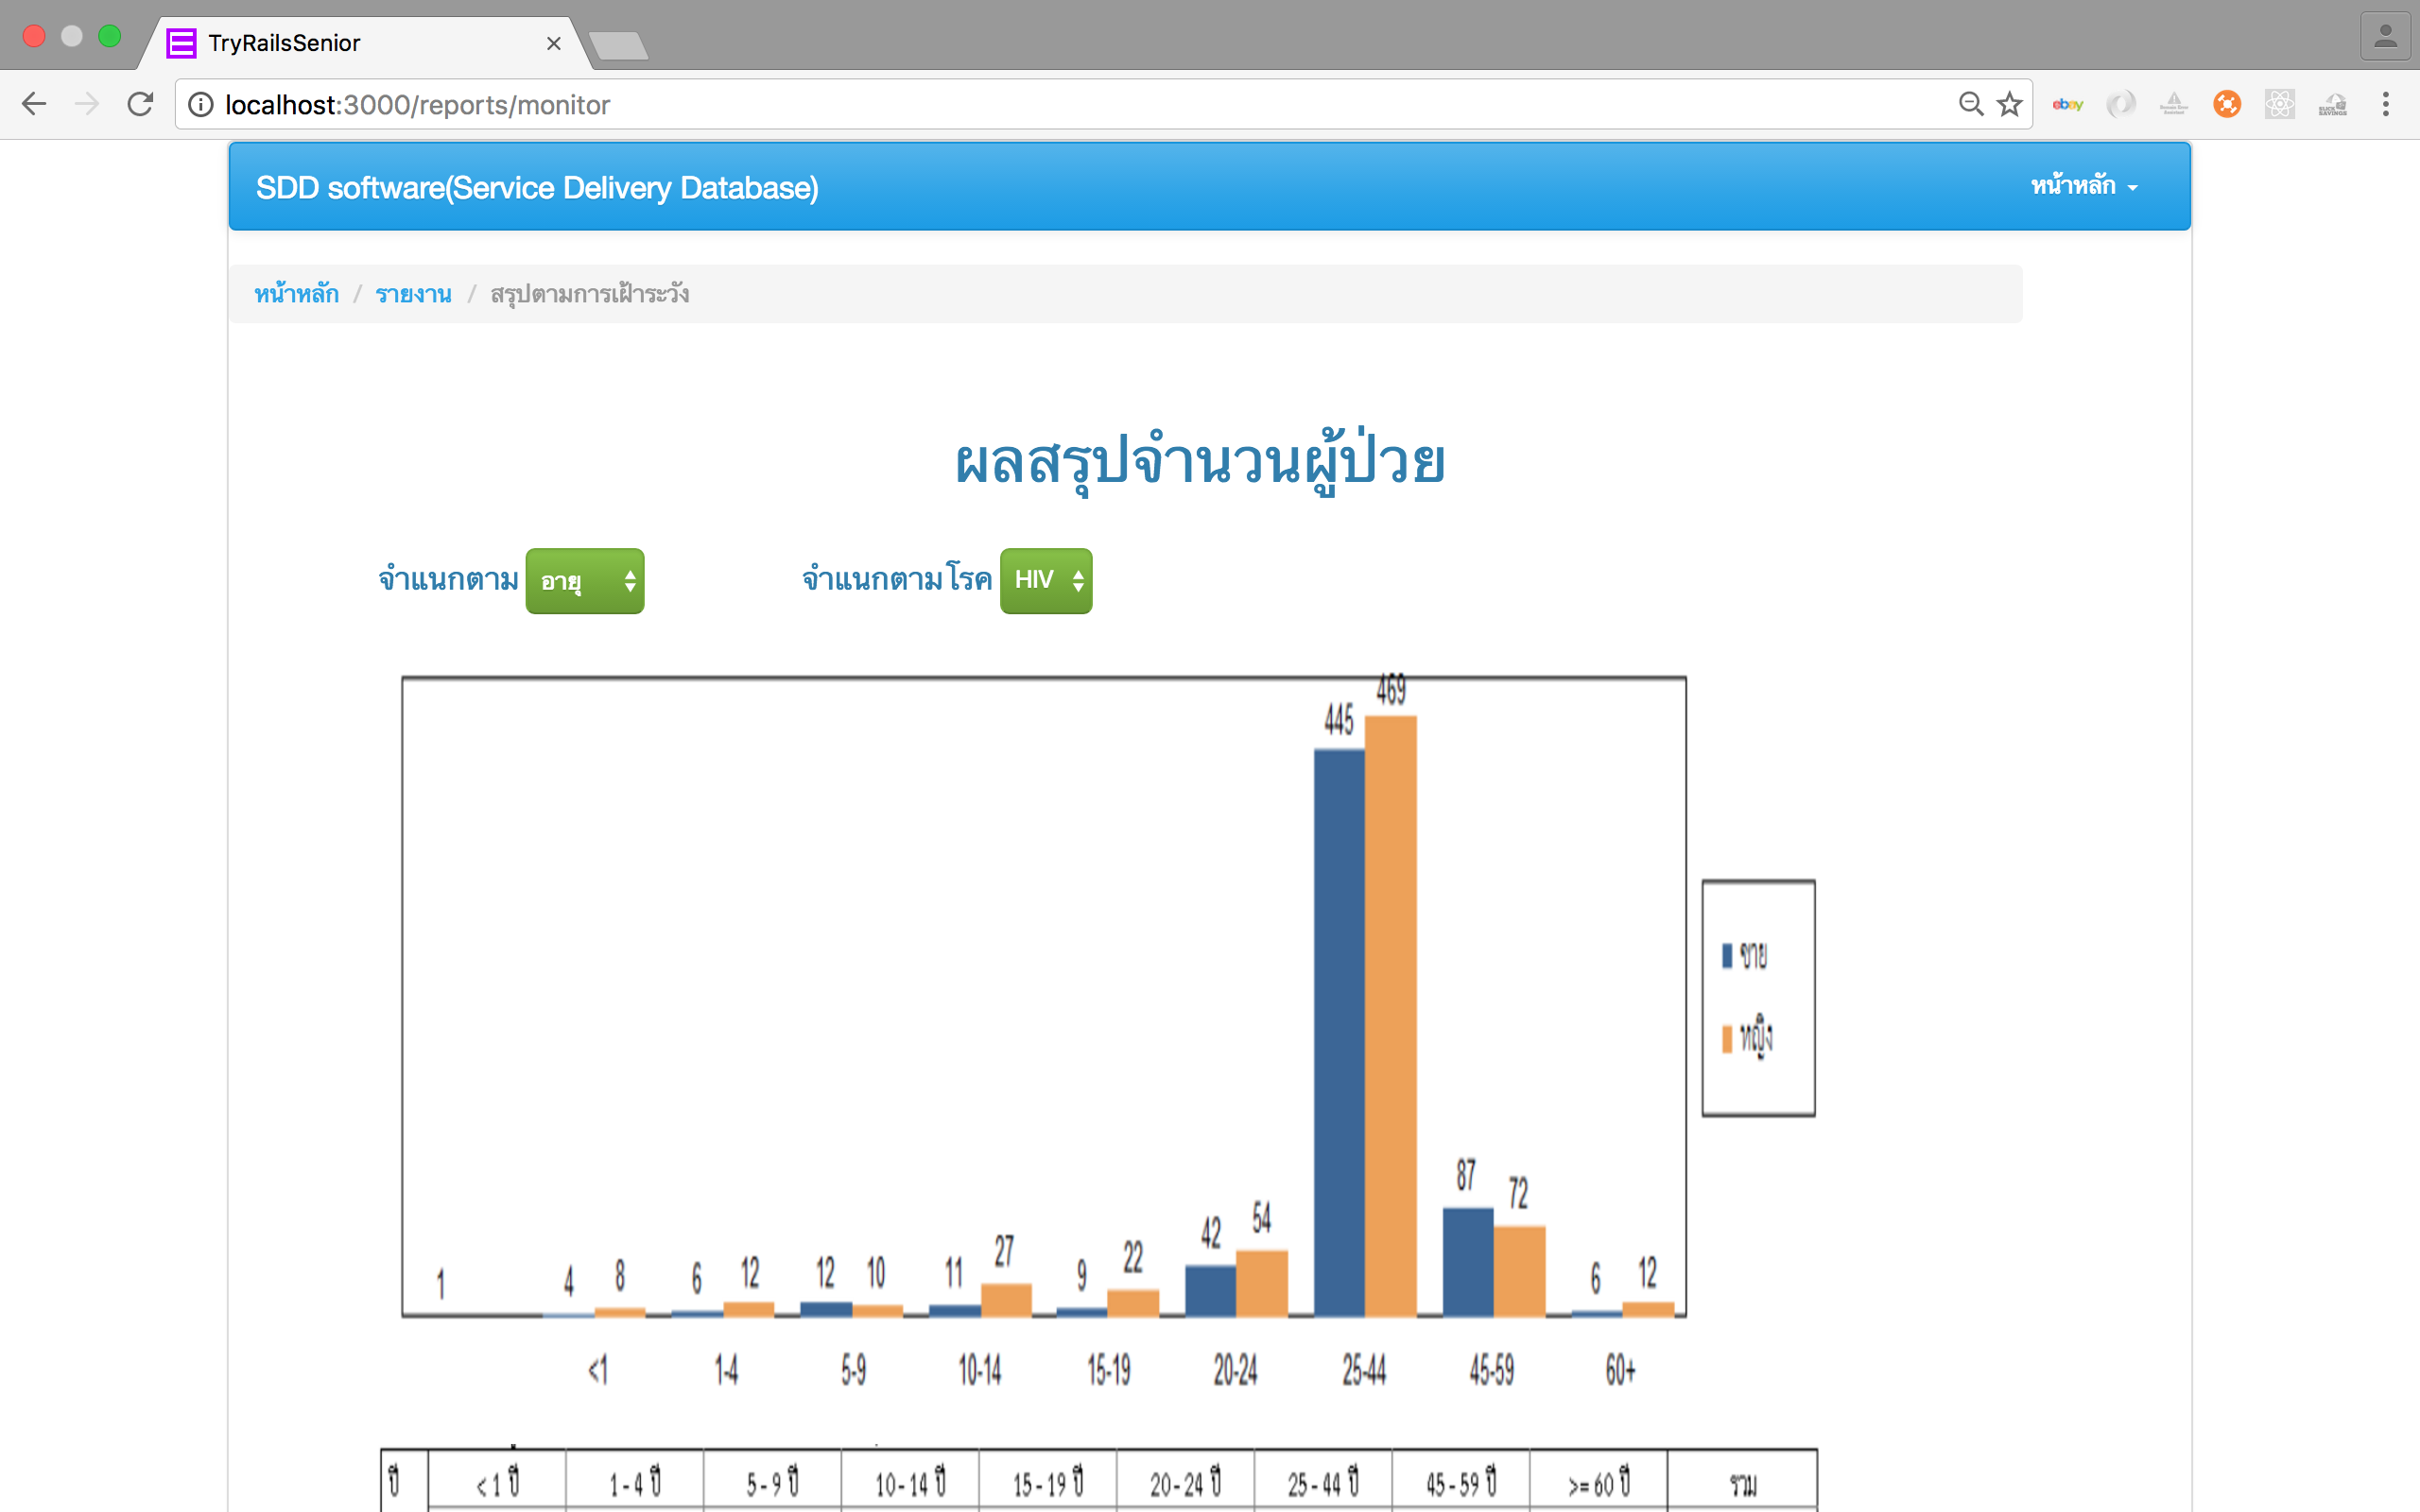
\includegraphics[width=12cm]{images/chapter-01/mockup_rails/report1.png}
                    	\caption{Monitor Report 1}
                    	\label{report1}
                \end{figure}
            \FloatBarrier
            
            \FloatBarrier
                \begin{figure}[h!]
                    \centering
                        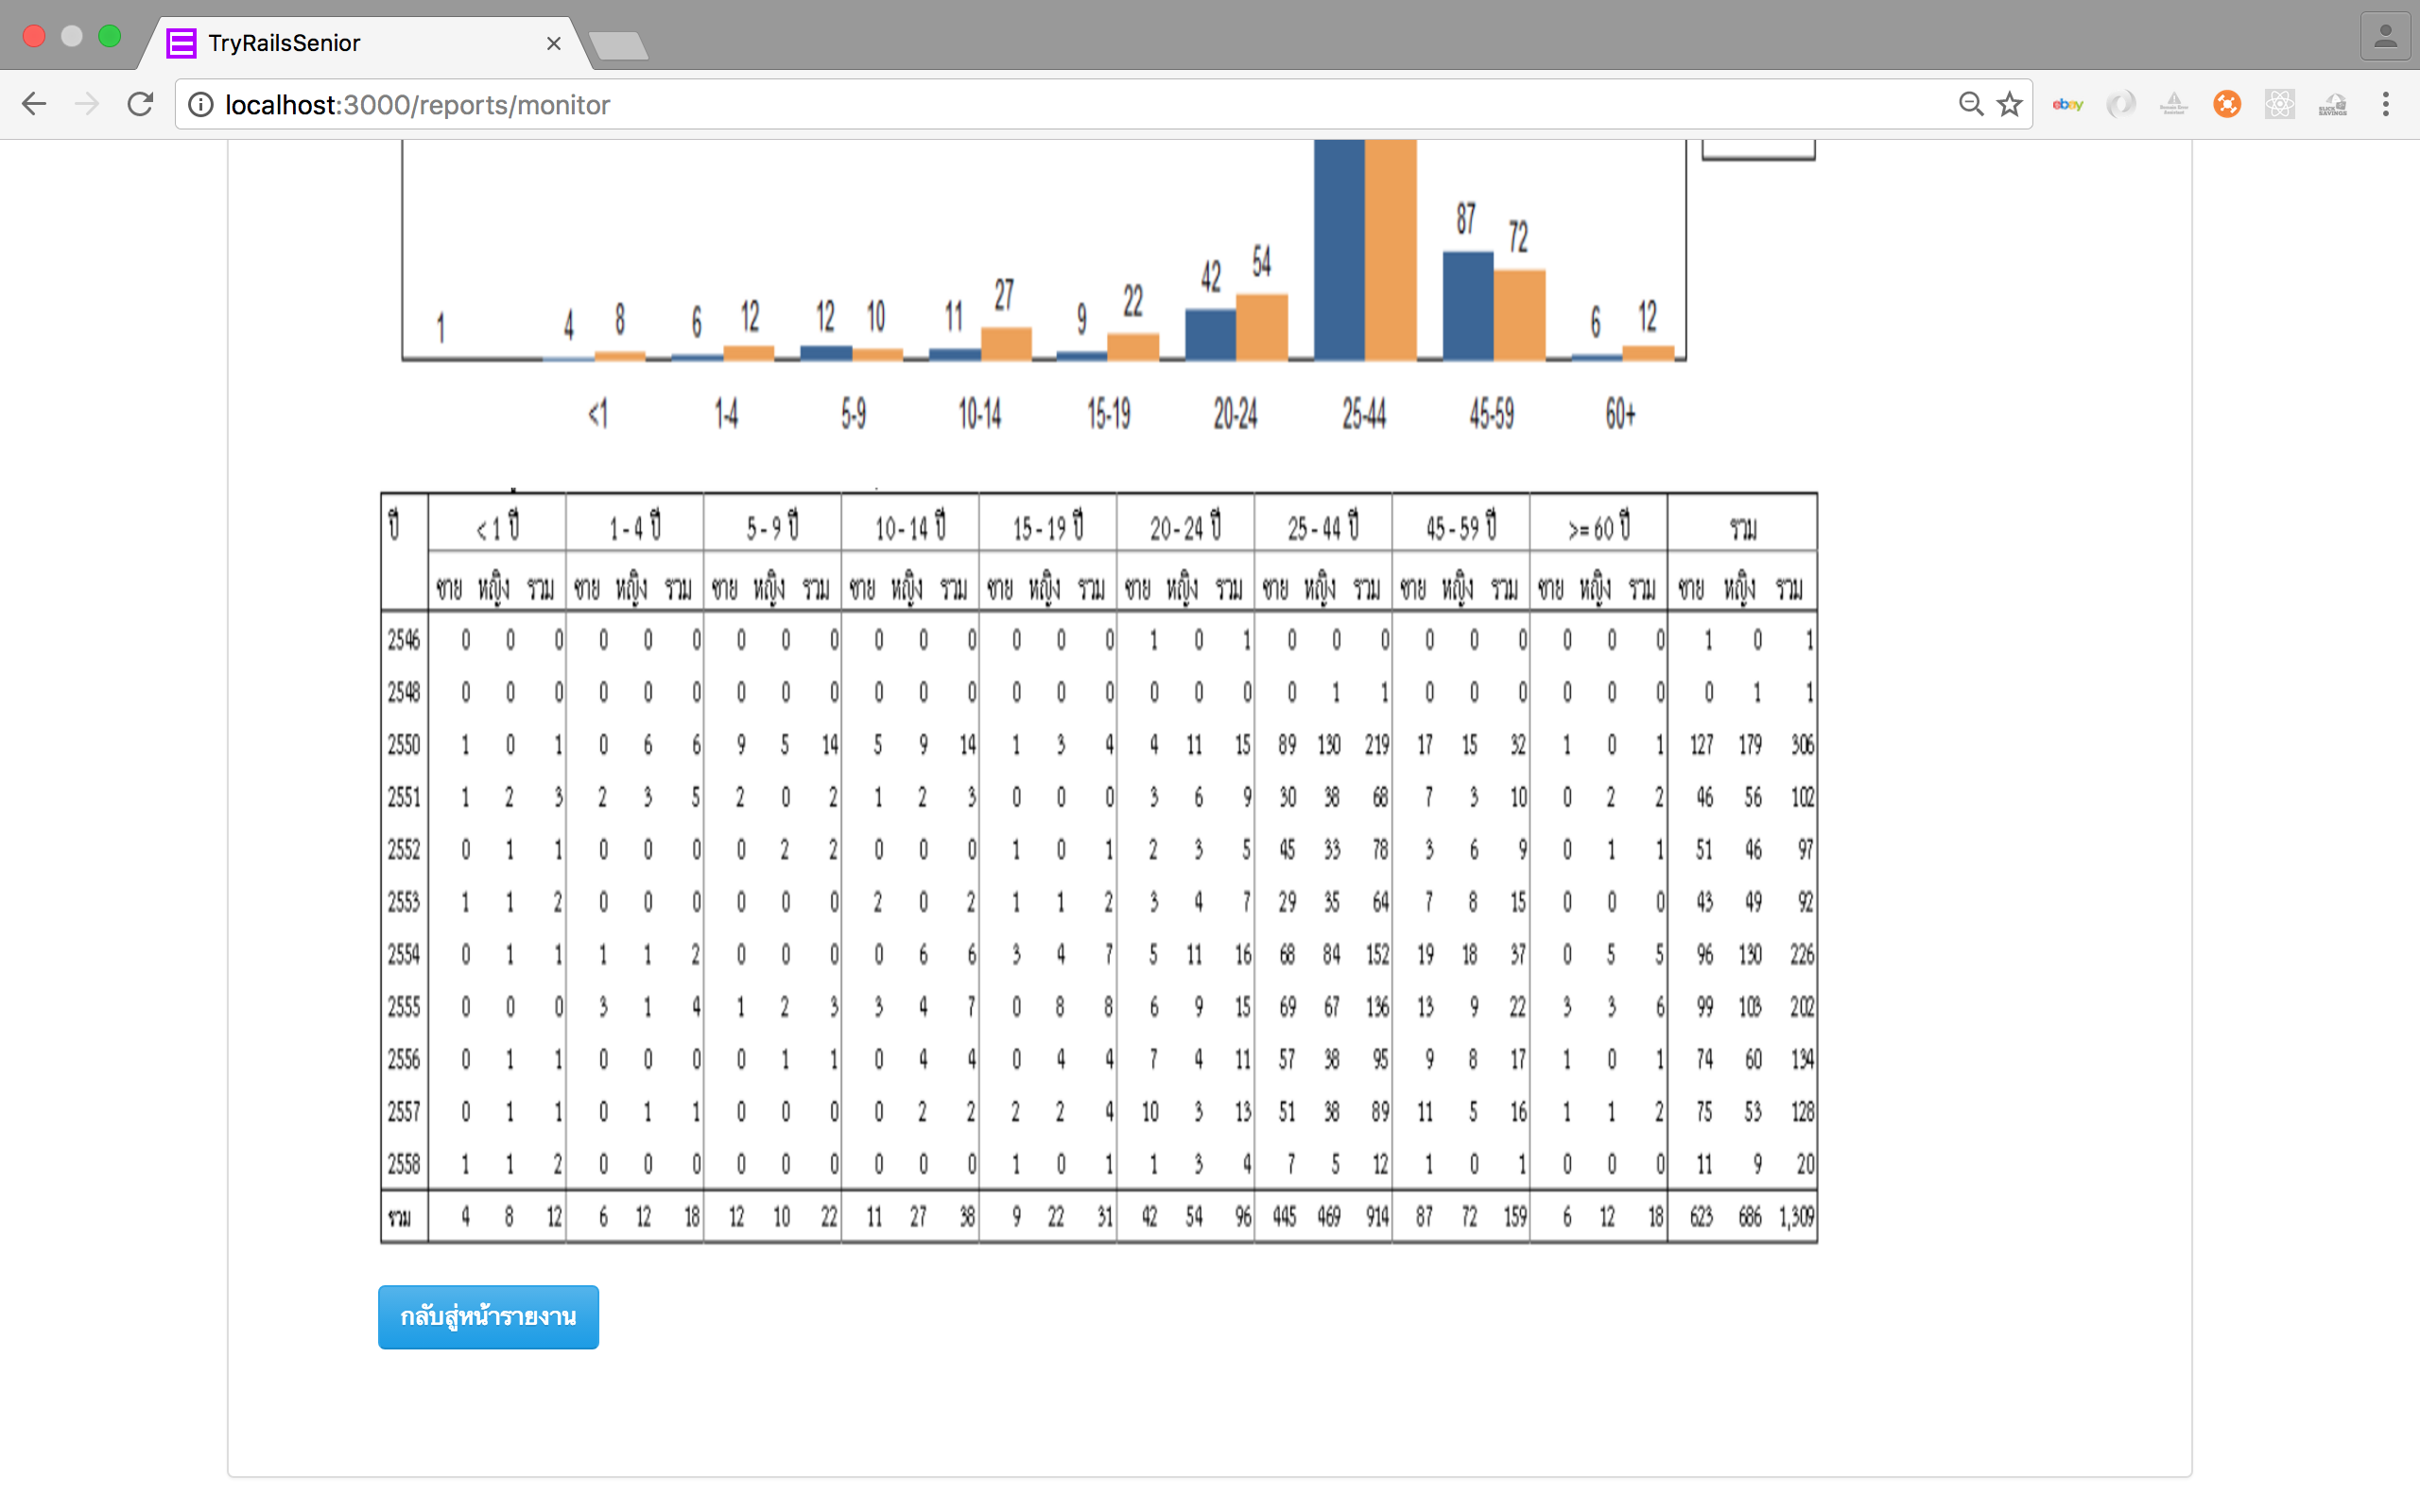
\includegraphics[width=12cm]{images/chapter-01/mockup_rails/report2.png}
                    	\caption{Monitor Report 2}
                    	\label{report2}
                \end{figure}
            \FloatBarrier


	

\section{Technologies}
    The following sections are the technologies and tools that we use for developing Epidemic Intelligent Information System.
    
    \subsection{Docker}
        Docker\cite{docker} is a software for automation deployment of the applications into containers. By using Docker containers, everything that is needed for the application to be able to run is packed into separated containers.
        
        In addition, Docker containers are not virtual machines. It does not need a separated operating system since it is built on top of Linux kernel. However, it depends on the functionality of the kernel and uses resource isolation (CPU, memory, block I/O, network, etc.). Because Docker containers are lightweight, we can run more applications on the server using Docker containers comparing to virtual machines.
        
    \subsection{MongoDB}
        MongoDB\cite{mongodb} is classified as NoSQL database which is an open source database that uses a document oriented data model. Instead of using tables and rows as relational database like SQL, MongoDB consist sets of key-value pairs , and collections are a set of documents and functions.  Like other NoSQL database, MongoDB uses a document storage format or we can call as BSON, which gives binary representation of JSON-like document. In addition, it also support dynamic schema design. In this system, we use MongoDB to store only the User data.
                
    \subsection{Nginx}
        Nginx\cite{nginx} is a web server. It can also be used for reverse proxy server, load balancer, and HTTP cache. In the system that we implemented, we use Nginx as a reverse proxy server for routing between our backend and frontend containers.
        
    \subsection{React}
        React\cite{react} is a javascript library for building interfaces which is maintained by Facebook. It is just a view layer in the application. There are several features in React. First, everything in React is component. The component mainly has state and props. The state is mutable while props is immutable meaning the value of state can be change over time while props can not be changed. This means it is one way data flow which make the behavior of the application predictable. Second, another feature of React is the use of "virtual Document Object Model" or "virtual DOM". The virtual DOM is used for efficient re-rendering of the DOM. This let the programmer to write code as if the entire page is rendered on each change of the data while the React renders only the subcomponent that only changes
        
    \subsection{Scalatra}
        Scalatra\cite{scalatra} is an open source web application framework which is written in scala. It is inspired from Sinatra framework which is implemented using Ruby. It is a microframework which gives developer more freedom because of its minimal.


% Should be on Deploy chapter???
% \section{Failure Handling}
%     Failure handling in this project is convenient since we containerized our application using Docker. There are restart policies\cite{docker_restart_policy} that Docker has provided. The restart policy that we are using in the system is "unless-stopped" which means it will always restart the container no matter the exit status is but it will not restart the container if the container is stopped by the user.